\documentclass{article}
\usepackage{graphicx}
\usepackage{hyperref}
\usepackage[a4paper, margin=1.25in]{geometry}
\usepackage{breakcites}
\usepackage{subcaption}
\usepackage{float}
\usepackage{textcomp}
\usepackage{amsmath}
\usepackage{textgreek}
\usepackage{authblk}
\usepackage{rotating}
\usepackage{booktabs}
\usepackage{longtable}
\usepackage{pdflscape}
\usepackage{lineno}
\usepackage[
  style=numeric,
  citestyle=numeric-comp,
  backend=biber,
  doi=true,
  natbib=true,
  sorting=none
]{biblatex}

\addbibresource{library.bib}

\begin{document}

\title{A Global Picture of Food Insecurity and Hunger}

\author[1,2,*]{Matthew Cooper}
\author[2,3]{Benjamin Müller}
\author[4]{Carlo Cafiero}
\author[2,5]{Juan Carlos Laso}
\author[2,6]{Wolfgang Fengler}
\author[2,7]{Homi Kharas}

\affil[1]{T.H. Chan School of Public Health, Harvard University}
\affil[2]{The World Data Lab, Vienna, Austria}
\affil[3]{Department of Economics, Vienna University of Economics and Business}
\affil[4]{The Food and Agricultural Organization of the United Nations}
\affil[5]{The International Institute for Applied Systems Analysis}
\affil[6]{The World Bank}
\affil[7]{The Brookings Institute}
\affil[*]{Corresponding Author: mcooper@hsph.harvard.edu}

\maketitle
\begin{abstract}
We modeled levels of of food security at a subnational level from 2010 to 2030 using microdata from 77 countries collected by the FAO and Gallup World Poll for the Voices of the Hungry project.  We find significant heterogeneity in levels of food security around the world, ranging from parts of the global north with less than 1\% of the population food insecure to parts of the global south where as much as 3 out of 4 people are severely food insecure.  Examining global temporal trends and accounting for the effects of the COVID-19 pandemic, we find that food insecurity has been increasing over the past several years, but under middle-of-the-road assumptions for development and population change, food insecurity will decline throughout the 2020s.  This global decrease is largely driven by trends in South and East Asia, and some parts of the world, particularly sub-Saharan Africa, are projected to show increases in the prevalence of food insecurity throughout the next decade. This is the first global picture at a subnational level of the Food Insecurity Experience Scale, the food security metric most indicative of the lived experience of hunger.
\end{abstract}

\section{Main}
Being food secure is a critical component of human flourishing, which is why the second Sustainable Development Goal (SDG 2) is ``Zero Hunger."  While a number of indicators are used to track progress towards this goal, the indicator that is most indicative of the human experience of food insecurity is the Food Insecurity Experience Scale, or FIES.  The FIES was developed due to a recognized need to measure actual food insecurity based on personal exposure to hunger, rather than proxies for food insecurity, such as estimates of calories per capita, or health consequences of food insecurity, such as child stunting.  However, as a relatively new metric, little work has been done so far to model food security or estimate current trends using the FIES at more local spatial scales.

Food security has traditionally been difficult to measure, and this has led to incomplete or inaccurate pictures of global hunger.  Metrics of macro-health, such as anthropometry and mortality rates are correlated broadly with food insecurity and have been used for many years to monitor human well-being \citep{Puffer1973, Habicht1974}.  However, these metrics are confounded with other determinants of health such as infectious disease and are not meaningful at the scale of individuals or households \citep{Perumal2018}.  Other proxies for food security, such as food availability estimated from crop yields \citep{Maxwell1992}, are also inadequate because they only make rough estimates of how accessible food is to the general population, and food insecurity can certainly occur in the absence of food availability decline \citep{Sen1983}.  Moreover, these metrics are very sensitive to incorrect estimates of crop yields and food reserves at a national scale.  Thus, global estimates of hunger and food insecurity based on these metrics carry forward similar flaws.

As researchers began to focus on food insecurity at the individual and household level, household microdata collecting information on household finances and consumption became a common proxy for food security \citep{Haddad1994}.  However, these efforts were criticized for being onerous, insufficiently comparable, as well as for ignoring subjective and experiential aspects of food security \citep{Maxwell1996}.  This led to the emergence of several indicators designed to be rapidly deployable, culturally cross-comparable, and based on the lived experience of food security \citep{Jones2013}.  These metrics include the Household Food Insecurity and Access Scale (HFIAS) \citep{Coates2007}; the Coping Strategies Index (CSI) \citep{Maxwell1999}; and the Household Hunger Scale (HHS) \citep{Ballard2011}.

Drawing on the insights derived in designing and implementing these novel food security metrics, the FIES was developed by the Food and Agricultural Organization (FAO) of the UN \cite{Ballard2013} and quickly became a useful tool for understanding individual and household-level food insecurity \citep{smith2017world}.  The FIES is based on a survey of eight behaviors indicative of food insecurity and hunger over the previous year, such as skipping meals or worrying about having enough to eat.  Using a Rash model \citep{Cafiero2018}, each individual in the survey is given a severity score, and thresholds for moderate and severe food insecurity are set at the behaviors of eating less than the respondent thought they should, and not eating for a while day, respectively.  Thus, people in moderate-to-severe food insecurity are estimated to have not eaten as much as they should have at least once in the previous year, while people in severe food insecurity are estimated to have gone an entire day without eating in the previous year.

Since 2014, in partnership with Gallup World Poll, the FAO has published surveys from around the world to estimate the prevalence of food insecurity using the FIES.  Drawing on surveys from 77 countries, we used machine learning to estimate levels of food insecurity around the world at the subnational level.  Our analysis highlights several important global and regional trends in food security.


\section{Results}
\subsection{Spatial Distribution of Food Insecurity}
We found significant heterogeneities in the global distribution of severe food insecurity, estimated to be people who had to go an entire day without eating at least once in the previous year (See Fig. \ref{fig:map}).  For the year 2020, mainland sub-Saharan Africa is the continent with with the highest rates of severe food insecurity, with at least 15\% of people in severe food insecurity in at last one region in every country except Gabon and Equatorial Guinea.  Outside of Africa, serious pockets of severe food insecurity also occur in Venezuela, Syria, Papua New Guinea, Yemen, and Afghanistan.  In many large middle-income countries, severe food insecurity is also quite prevalent, with rates between 10-15\% in areas like northern Brazil, many central Asian and middle-eastern countries, and India and Indonesia.

The experience of at least moderate food insecurity, or eating less than one would prefer, is quite common in many parts of the world.  In 2020, it is quite common in Africa, south and southeast Asia, and parts of Latin America, where in many places over 50\% of the population experiences this degree of food insecurity.  Even in countries widely considered to be developed, such as Australia, the United States, and parts of eastern and southern Europe, moderate-to-severe food insecurity is as high as 10-15\%.  

\begin{landscape}
\begin{figure}[h]
  \centering
  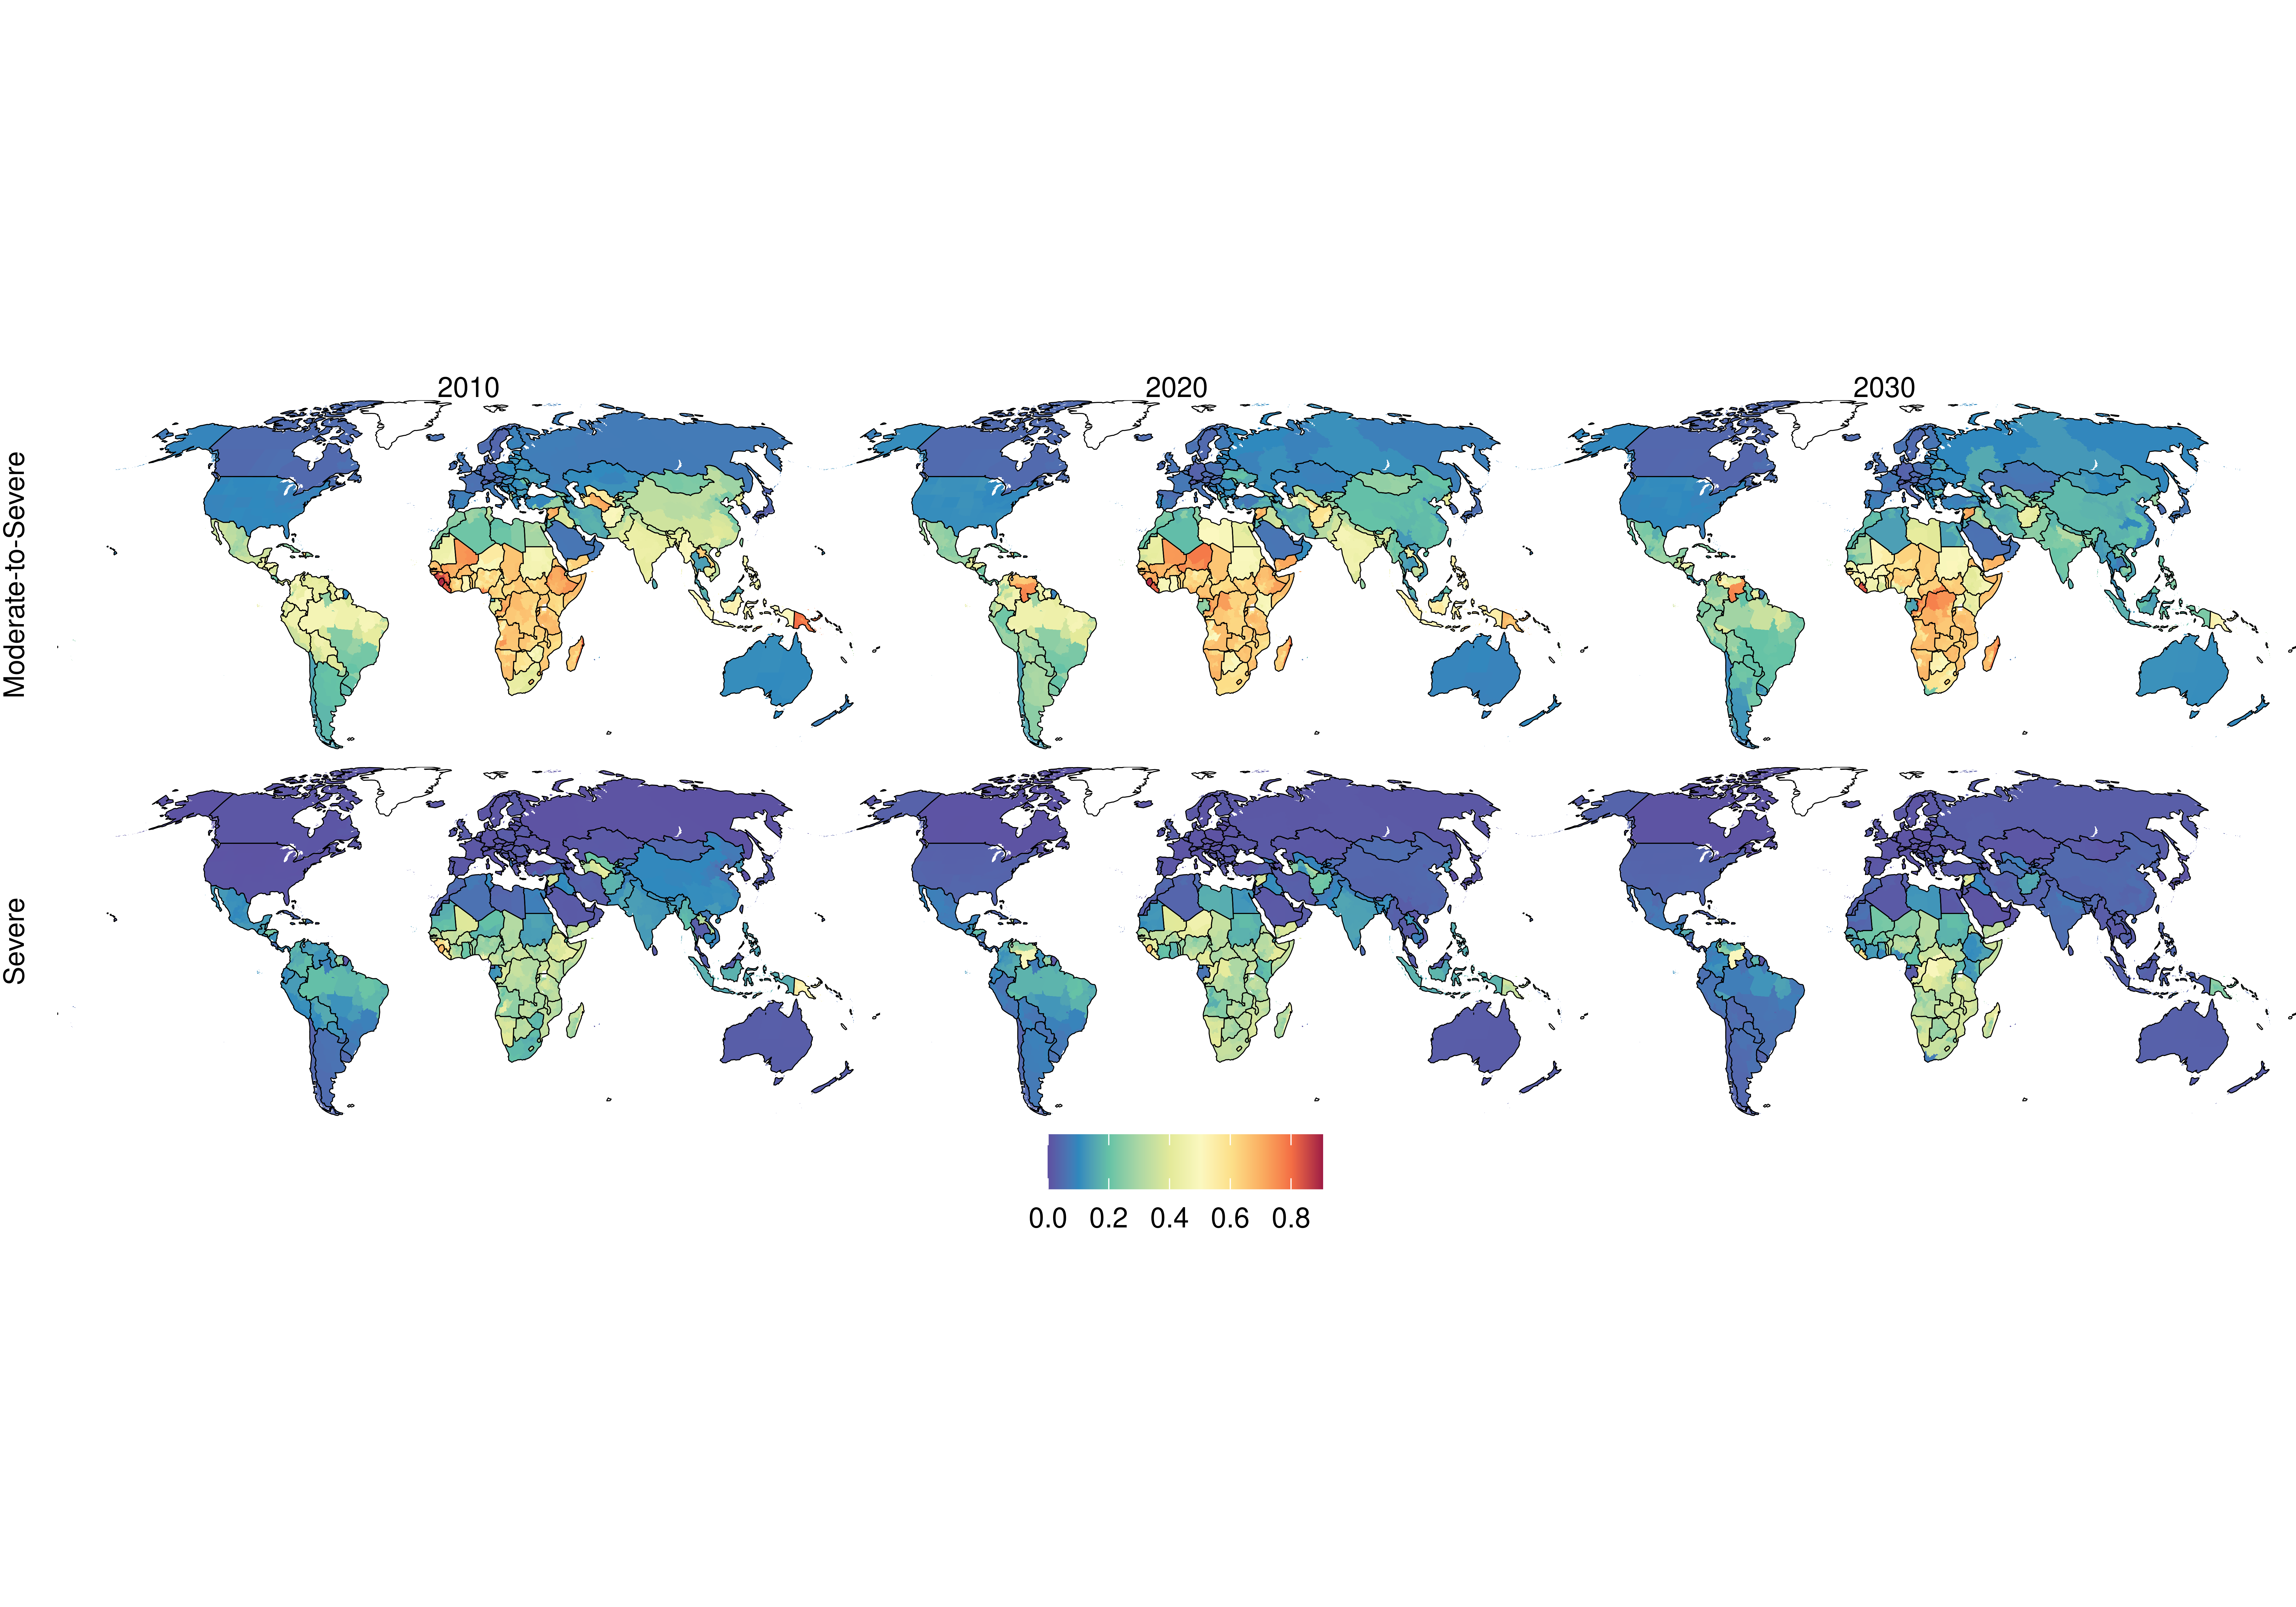
\includegraphics{img/FullMap.pdf}
  \caption{Modeled rates of severe and moderate-to-severe food insecurity for the years 2010, 2020, and 2030}
  \label{fig:map}
\end{figure}
\end{landscape}

Globally, in the year 2020, we estimate that 2.33 billion people experience at least moderate food insecurity, and 829 million people experience severe food insecurity (See Fig. \ref{fig:timeseries}).  While the total number of people in moderate and severe food security held roughly constant for the 2010s and even increased in latter part of that decade, we predict that it will decline throughout the 2020s.  However, this overall decline will not be uniform across the world.  Our model expects that, in most of sub-Saharan Africa, moderate food insecurity will increase throughout the 2020s and severe food insecurity will plateau, although some countries, such as Kenya, Ethiopia, and Ghana, will see improvements.  Food Security will fall in most other world regions, particularly South Asia and East Asia \& the Pacific.  

\begin{figure}[H]
  \centering
  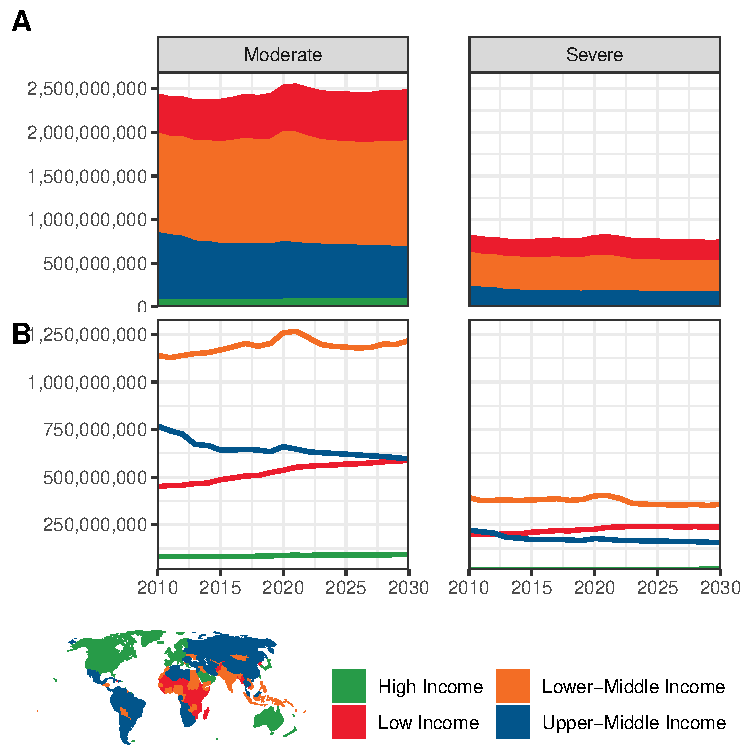
\includegraphics[width=\linewidth]{img/TimeSeries.pdf}
  \caption{Number of people in moderate-to-severe and severe food insecurity, by World Bank regions over time, with a 3-year smoothing.  Panel (A) shows the number of food insecure people with region totals stacked, to show global trends and totals over time.  Panel (B) shows regional totals compared against each other over time.}
  \label{fig:timeseries}
\end{figure}

This results of this analysis can be explored in more detail on the \href{worldhunger.io}{World Hunger Clock}, including statistics for each subnational administrative area.


\section{Discussion}
This paper presents the first global estimates of the experience of food insecurity at a subnational level, with forecasts out to the year 2030.  We found that, while food insecurity has been increasing and has worsened in 2020 with the novel coronavirus, our models predict that number of people who experience food insecurity globally will decrease throughout the 2020s, largely because of progress in south and east Asia.  Nevertheless, many regions, most notably sub-Saharan Africa, are expected to see overall increases in the number of food insecure people.

While this is the first comprehensive projection of indicator 2.1.2 for SDG 2, projections for other indicators for that goal have been made.  The most recent State of Food Insecurity (SOFI) report by the FAO projected indicator 2.1.1, the prevalence of undernourishment, and found that that, much like food insecurity, undernourishment had been increasing throughout the 2010s \citep{sofi2020}.  The SOFI report also modeled the prevalence of undernourishment in 2030 based on recent trends, giving more weight to recent years, and projected that undernourishment will increase by 2030 \citep[Part 1, Page 11]{sofi2020}.  Using a similar method for modeling the prevalence of stunting (indicator 2.2.1), the SOFI reported that the rate of stunting would decrease by 2030 \citep[Part 1, Page 30]{sofi2020}.

The fact that the SOFI expects increases in undernourishment while we predict decreases in food insecurity is likely due to our differing modeling approaches. While the SOFI report extrapolated recent trends in undernourishment, we modeled food insecurity based on projections of factors like GDP per capita, population, and the prevalence of stunting.  We found that, in a random forest model, these predictors were very successful at predicting recent rates of both moderate-to-severe and severe food insecurity.

While we found that food insecurity will decrease overall by 2030, our middle-of-the-road scenario only expects the number of people experiencing moderate or severe food insecurity to fall by 12\% and the number of people experiencing severe food insecurity to fall by 20\%.  This still leaves billions of people eating less than they should and nearly half a billion people going entire days without eating a decade from now, far short of the SDG 2 goal of ``zero hunger."  Moreover, decreases in food insecurity as measured by the FIES do not necessarily mean there will be improvements in other significant challenges such as poor dietary quality, micronutrient deficiencies, or obesity.  Thus, while expected trends in correlates of food security give cause for optimism, there is still significant work to be done in pursuit of SDG 2.

\section{Methods}

\subsection{Disaggregation}
The data on the FIES collected by Gallup records many individual-level attributes from the respondents, including age, gender, wealth quintile, and whether they live in an urban or rural area.  Using national data on these variables, a standard weighting schema is created for each individual, based on the ratio of population probabilities to sample probabilities of an individual with those characteristics being selected \citep{bethlehem2009applied}.  We used a similar methodology, except we calculated post-stratification weights at a subnational level.  We used year-specific subnational estimates of population percentages by gender, age, urbanization, and, where available, wealth, and created a separate set of weights for each admin area across all individuals.  For age and gender, we used gridded data from WorldPop \citep{Tatem2017}, for urbanization, we used spatially explicit estimates published by Jones and O'Neill \citep{Jones2016}, and for wealth we used data from Demographic and Health Surveys \citep{dhsall}.  This methodology rests on the mild assumption that subnational differences in rates of food insecurity are more due to factors related to demographics, urbanization, and wealth than to other unobservable factors.

\subsection{Covariates}
We model subnational rates of severe and moderate-to-severe food insecurity as a function of several covariates related to human development, food security, health, infrastructure, and the environment (See Table \ref{tab:covars}).  We aimed for covariates that had subnational spatial resolution and peer-reviewed projections available through the year 2030.  For many variables, we combined historic subnational data with national projections through the 2020s to derive simple subnational estimates for the next decade.  For projections based on the Shared Socioeconomic Pathways (SSP) framework, we used the middle-of-the-road pathway, SSP2, and for climatological variables, we use forecasts based on Representative Concentration Pathway (RCP) 6.0.  Finally, we adjusted several variables to account for the effects of COVID-19, including GDP per capita using June 2020 estimates from the World Bank \citep{prospects2020}, stunting and wasting using August 2020 estimates published in \textit{The Lancet} \citep{headey2020impacts}, as well as the poverty headcount index \cite{cuaresma2018will}.  For a detailed overview of the steps involved in processing and preparing each covariate, see the Appendix.


\begin{table}[H]
  \centering
	\begin{tabular}{ll}
		\toprule
		Name & Source \\
		\midrule
		Urban Percentage & \citep{Jones2016} \\
		Stunting & \citep{Local2020} \\
		Wasting & \citep{Local2020} \\
		Mean Years of Schooling & \citep{Smits2019, KC2017} \\
		GDP Per Capita & \citep{Smits2019, Dellink2017} \\
		Gini Coefficient & \citep{Rao2019a} \\
    Poverty Headcount Index & \citep{Cuaresma2018} \\
		Water Scarcity & (CITATION) \\
		Mean Annual Precipitation &  \cite{abatzoglou2018terraclimate, warszawski2014inter} \\
		Topographic Ruggedness &  \cite{USGS1996, Riley1999} \\
		Mean Temperature &  \cite{abatzoglou2018terraclimate, warszawski2014inter} \\
		Malaria (\textit{P. falciparum}) Mortality Rate &  \cite{Weiss2019} \\
		\bottomrule
	\end{tabular}
	\caption{Covariates Included in Present-Day Analysis}
	\label{tab:covars}
\end{table}


\subsection{Modeling}

We modeled subnational rates of moderate-to-severe and severe food insecurity globally at the subnational level in the period of 2010 to 2030 using the disaggregated FIES data combined with the covariates. Using the log-transformed rate of food insecurity as our outcome variable, we explored several modeling approaches, including linear regression methods such as Least Absolute Shrinkage and Selection Operator (LASSO) regression and Bayesian Stochastic Search and Variable Selection (Bayes SSVS), as well as machine learning methods such as Random Forest regression. 

Based on various model validation metrics, Random Forest (RF) regression performed the best. The RF regression involves generating a large number of decision trees, each under slightly different conditions and using different sub-samples of the data, and then aggregating the predictions of the decision trees.  Random forest models are known to perform well in the presence of non-linearities and important interactions among predictor variables \citep{breiman2001random}. Since this is likely to be the case in our application, this method is particularly suitable for modeling rates of moderate-to-severe and severe food insecurity. 

We observed for the moderate-to-severe as well as the severe RF regression model an in-sample mean squared error (MSE) between 0.002-0.005, with a R-squared (${R}^2$) value of 0.999 (See Fig. \ref{fig:rf_in-sample}). Although RF regression models tackle the issue of overfitting by applying various ensemble methods \citep{breiman2001random}, it is crucial to validate the out-of-sample prediction performance. Hence, we trained the RF regression model with 75\% of the available observations and predicted rates of moderate-to-severe and severe food insecurity for the remaining 25\%. Similarly to the in-sample model validation metrics, the out-of-sample MSE is between 0.008-0.017, with a ${R}^2$ of around 0.98-0.99 for both models (See Fig. \ref{fig:rf_out-sample}).

To get the best possible model performance, it is necessary to tune the hyperparamters, which control the process in which the random forest algorithm is run.  Key hyperparameters include the number of decision trees to generate, the number of variables randomly selected as candidates for splitting a node, and the average number of observations in a leaf node.  We calculated the Out-Of-Bag (OOB) error for different combinations of hyperparameters for the moderate-to-severe and severe models. By choosing the combination of hyperparameters with the smallest OOB error we found the optimal combination for both models respectively. We found that 5000 trees are more than sufficient for the error rates to converge (See Fig. \ref{fig:rf_error}).

Apart from tuning the hyperparameters, we examined the importance of the individual covariates in explaining rates of moderate-to-severe and severe food insecurity. By training the models with all covariates and predicting rates with and without a individual variable we calculated the average prediction error of omitting that variable. Using the highest average prediction error we ranked the importance of the variables and found that for both, the moderate-to-severe and severe model, the Poverty Headcount Index, Stunting, GDP Per Capita and the Gini Coefficient are the most important variables for explaining differences in rates of moderate-to-severe and severe food insecurity (See Fig. \ref{fig:rf_vimp}).

For a detailed description, implementation and validation of the RF regression models see the Supplemental Info.

\section{Conclusion}

\printbibliography

\section*{Supplemental Info}
\setcounter{table}{0}
\setcounter{figure}{0}
\setcounter{section}{0}
\renewcommand{\thetable}{S\arabic{table}}
\renewcommand{\thefigure}{S\arabic{figure}}
\renewcommand{\thesection}{S\arabic{section}}

\section{Component Questions of the FIES}
\begin{enumerate}
	\item During the last 12 MONTHS, was there a time when you were worried you would not have enough food to eat because of a lack of money or other resources?
	\item Still thinking about the last 12 MONTHS, was there a time when you were unable to eat healthy and nutritious food because of a lack of money or other resources?
	\item Was there a time when you ate only a few kinds of foods because of a lack of money or other resources?
	\item Was there a time when you had to skip a meal because there was not enough money or other resources to get food?
	\item Still thinking about the last 12 MONTHS, was there a time when you ate less than you thought you should because of a lack of money or other resources?
	\item Was there a time when your household ran out of food because of a lack of money or other resources?
	\item Was there a time when you were hungry but did not eat because there was not enough money or other resources for food?
	\item During the last 12 MONTHS, was there a time when you went without eating for a whole day because of a lack of money or other resources?
\end{enumerate}

\section{Predicting Covariates Into the Future}
\subsection{Annualized Rate of Change}
For many of our covariates, to extrapolate recent trends to the future, it is necessary to draw on annualized rates of change, which are then used to anticipate the rate of future change.  This method can be used for any variable that is a fraction or a rate.  We use this method to estimate future rates of stunting, wasting, and malaria mortality, as well as to model future admin shares of GDP and population.  Thus, we give an overview of the methodology here.

First, for each admin area, $a$, the rate of change (ROC) is calculated between each pair of adjacent years, $y$, based on a value, $p$, such that $0 < p < 1$, available for each year.

\begin{equation}
  \text{ROC}_{a,y} = \text{logit} \left( \frac{p_{a,y}}{p_{a,y-1}} \right)
  \label{eqn:a}
\end{equation}

Then, each ROC is weighted to give more weight to recent years, such that weight $W$ at year $y$ is.  For a dataset with observations for 2010 to 2017, that would be:

\begin{equation}
  W_y = \frac{y - 2010}{\sum_{y=2010}^{2017} y - 2010}
  \label{eqn:b}
\end{equation}

Then, the annualized rate of change (AROC) is calculated as:

\begin{equation}
  \text{AROC}_{a} = \text{logit} \left( \sum_{y=2010}^{2017} W_y \times \text{AROC}_{a, y} \right)
  \label{eqn:c}
\end{equation}

Finally, the projections, Proj, for each year from 2018 to 2030 are given as:

\begin{equation}
  \text{Proj}_{a,y} = \text{logit}^{-1} ( \text{logit} ( p_{a,2017} ) + AROC_{a} \times ( y - 2017 ) )
  \label{eqn:d}
\end{equation}

For cases where we are modeling shares of a whole, for example when modeling subnational shares of population or GDP, we then re-scale the shares to ensure they total to 1.

\subsection{Population}
Although population is not a covariate in our random forest model, it is an important precursor to other covariates, such as GDP per capita, and future estimates of population are also necessary to convert modeled future rates of food insecurity into total headcounts of food insecurity.  Thus, in addition to our other covariates, we also modeled population into the future.

We do this by combining historic subnational data from the Subnational Development Database \citep{Smits2019} with national level population estimates for the 21st century \citep{KC2017}.  To account for within-country trends and changes in population distribution, we use the AROC method outlined in equations \ref{eqn:a} - \ref{eqn:d} to project each admin areas share of national population totals. We then disaggregate the national totals given by KC et al. to estimate future subnational populations.

\begin{figure}[H]
  \centering
  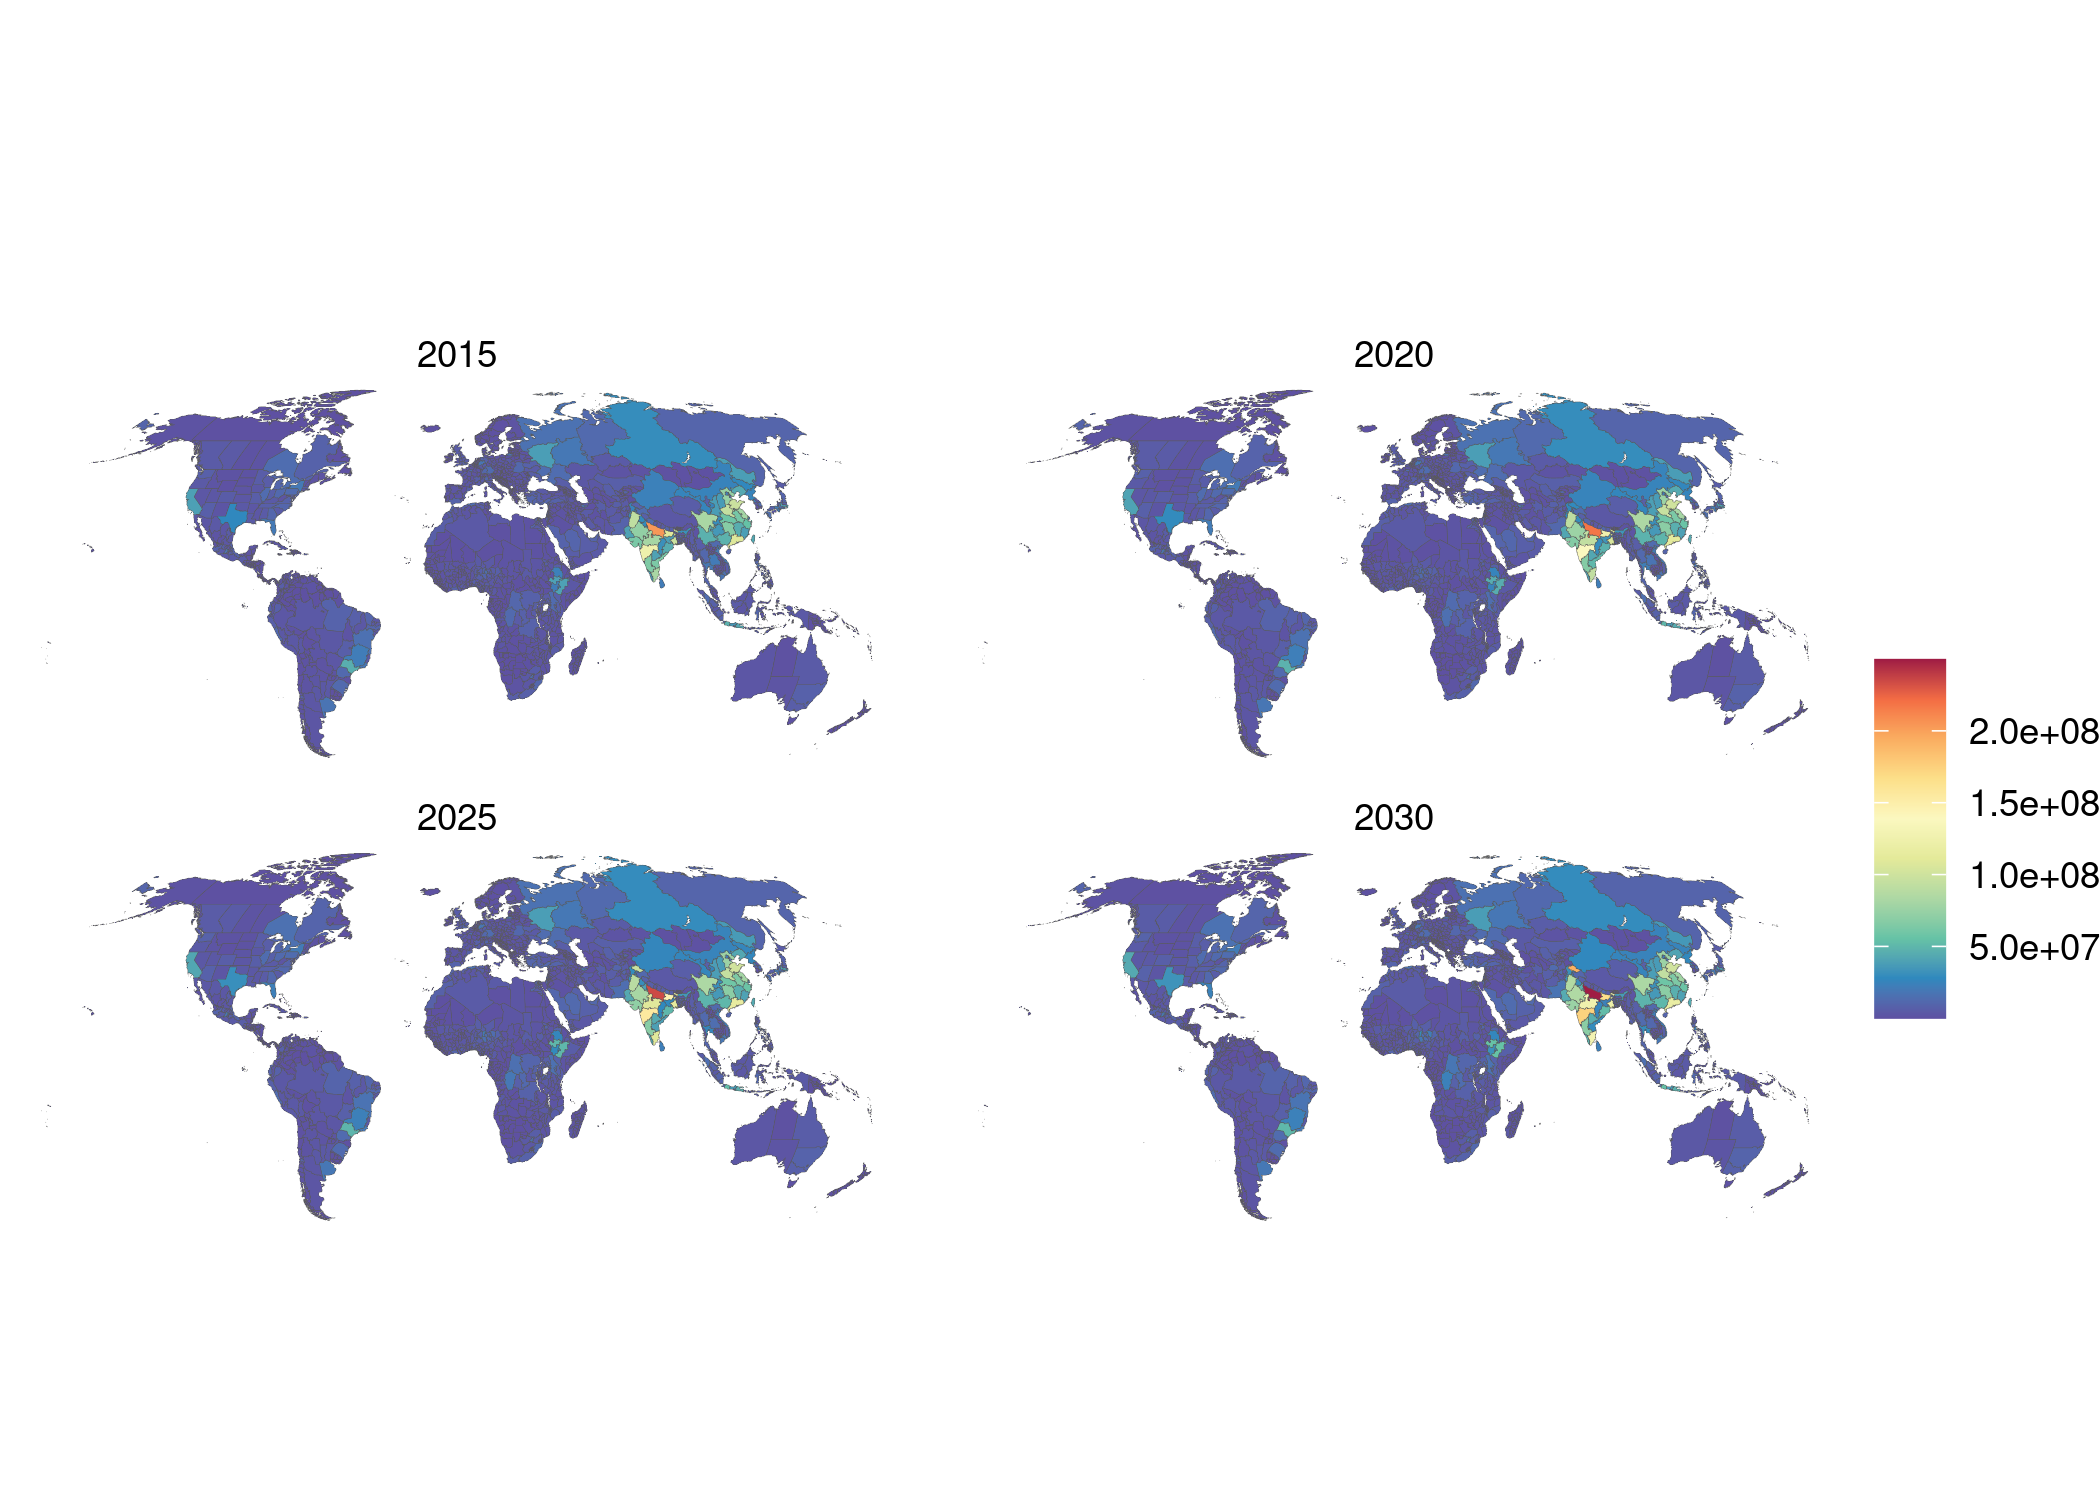
\includegraphics[width=\linewidth]{img/covars/population.png}
  \caption{Population}
\end{figure}

\subsection{Urban Percentage}

We drew our historic and future estimates of urbanization entirely from Jones and O'Neill, published in \textit{Environmental Research Letters} \citep{Jones2016}, who modeled spatially explicit scenarios of urbanization consistent with the Shared Socioeconomic Pathways.  As with our other covariates, we used estimates for SSP2, the middle-of-the-road scenario.  Because definitions of ``urban" and ``rural" vary significantly across datasets, using one dataset that is entirely consistent within itself was an important consideration.

\begin{figure}[H]
  \centering
  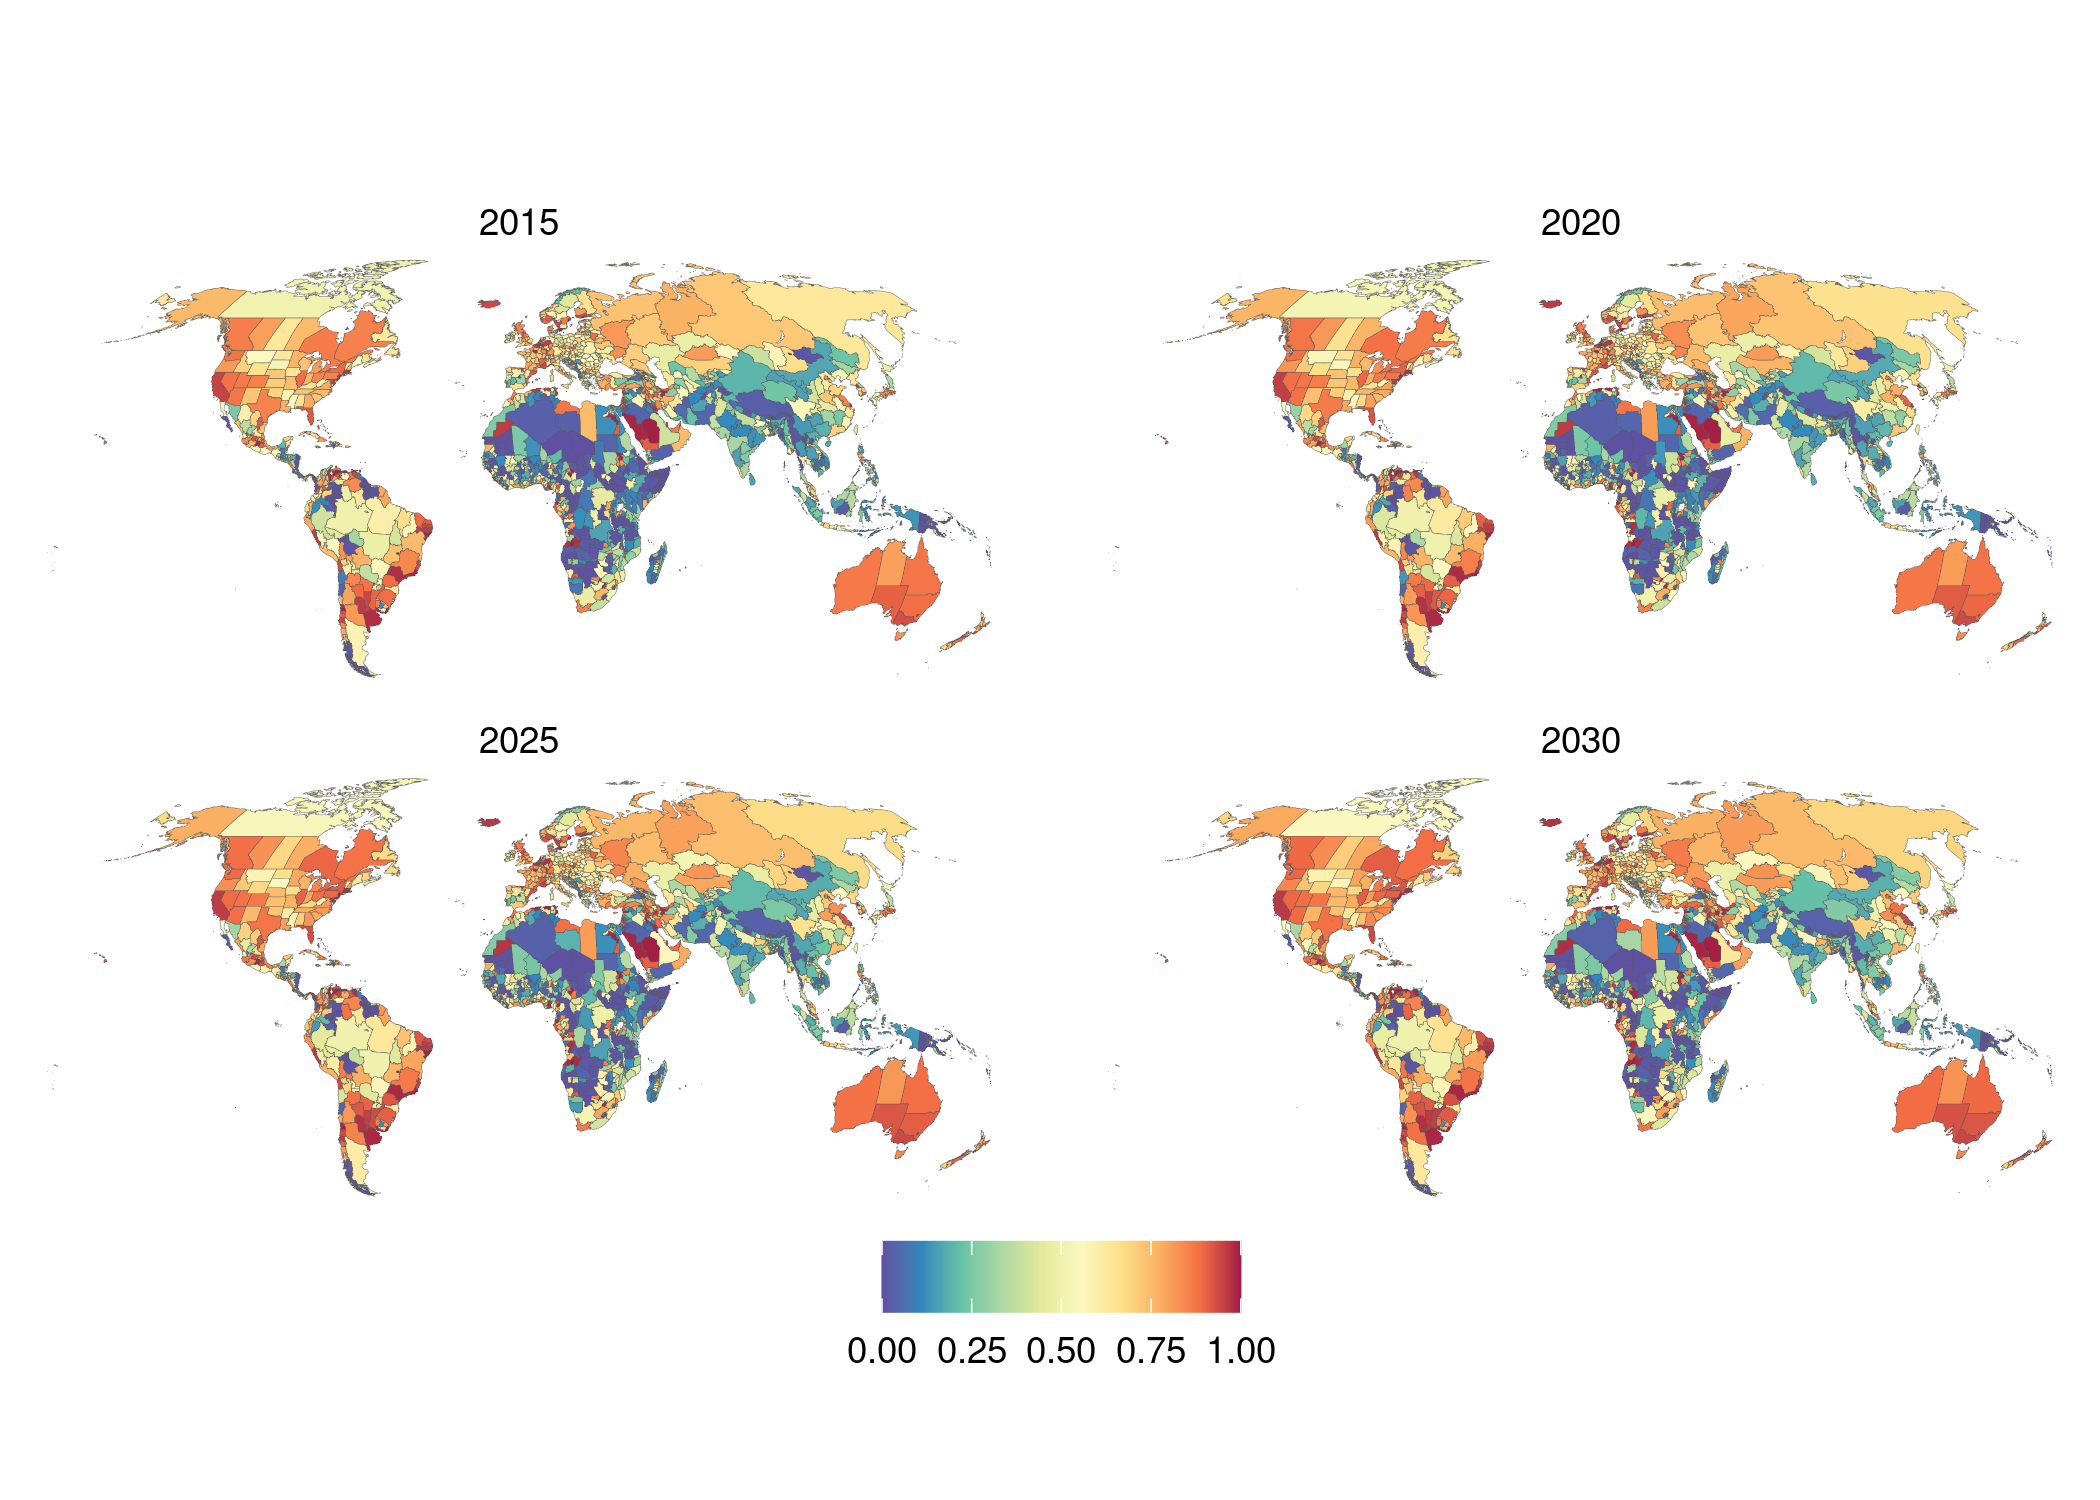
\includegraphics[width=\linewidth]{img/covars/urban_perc.png}
  \caption{Percentage of people living in urban areas.}
\end{figure}

\subsection{Wasting}
To estimate the prevalence of wasting for each administrative area in our dataset, we used data from the Local Burden of Disease project published in \textit{Nature} \citep{Local2020}.  For the years 2010 to 2017, we simply took the mean rate of wasting in each administrative area from the dataset.  Higher-income countries that were not included in the dataset were modeled as having a rate of 0 wasting.  We then modeled wasting for the years 2018-2030 using the AROC method, which the Local Burden of Disease group similarly used to estimate wasting for the year 2025 \citep{Local2020}.

To account for the effects of the novel coronavirus on global rates of wasting, we assumed that long-term trends and rates of wasting would hold steady, but that they increase globally by 14.3\% in 2020, based on estimates published in \textit{The Lancet} \citep{headey2020impacts}.  We model this impact as uniform across all countries where wasting occurs.  Then we model the rate of wasting in each administrative area in 2021 as being the mean of the rate in 2020 that accounts for the shock and the previously modeled rate for 2022.

\begin{figure}[H]
  \centering
  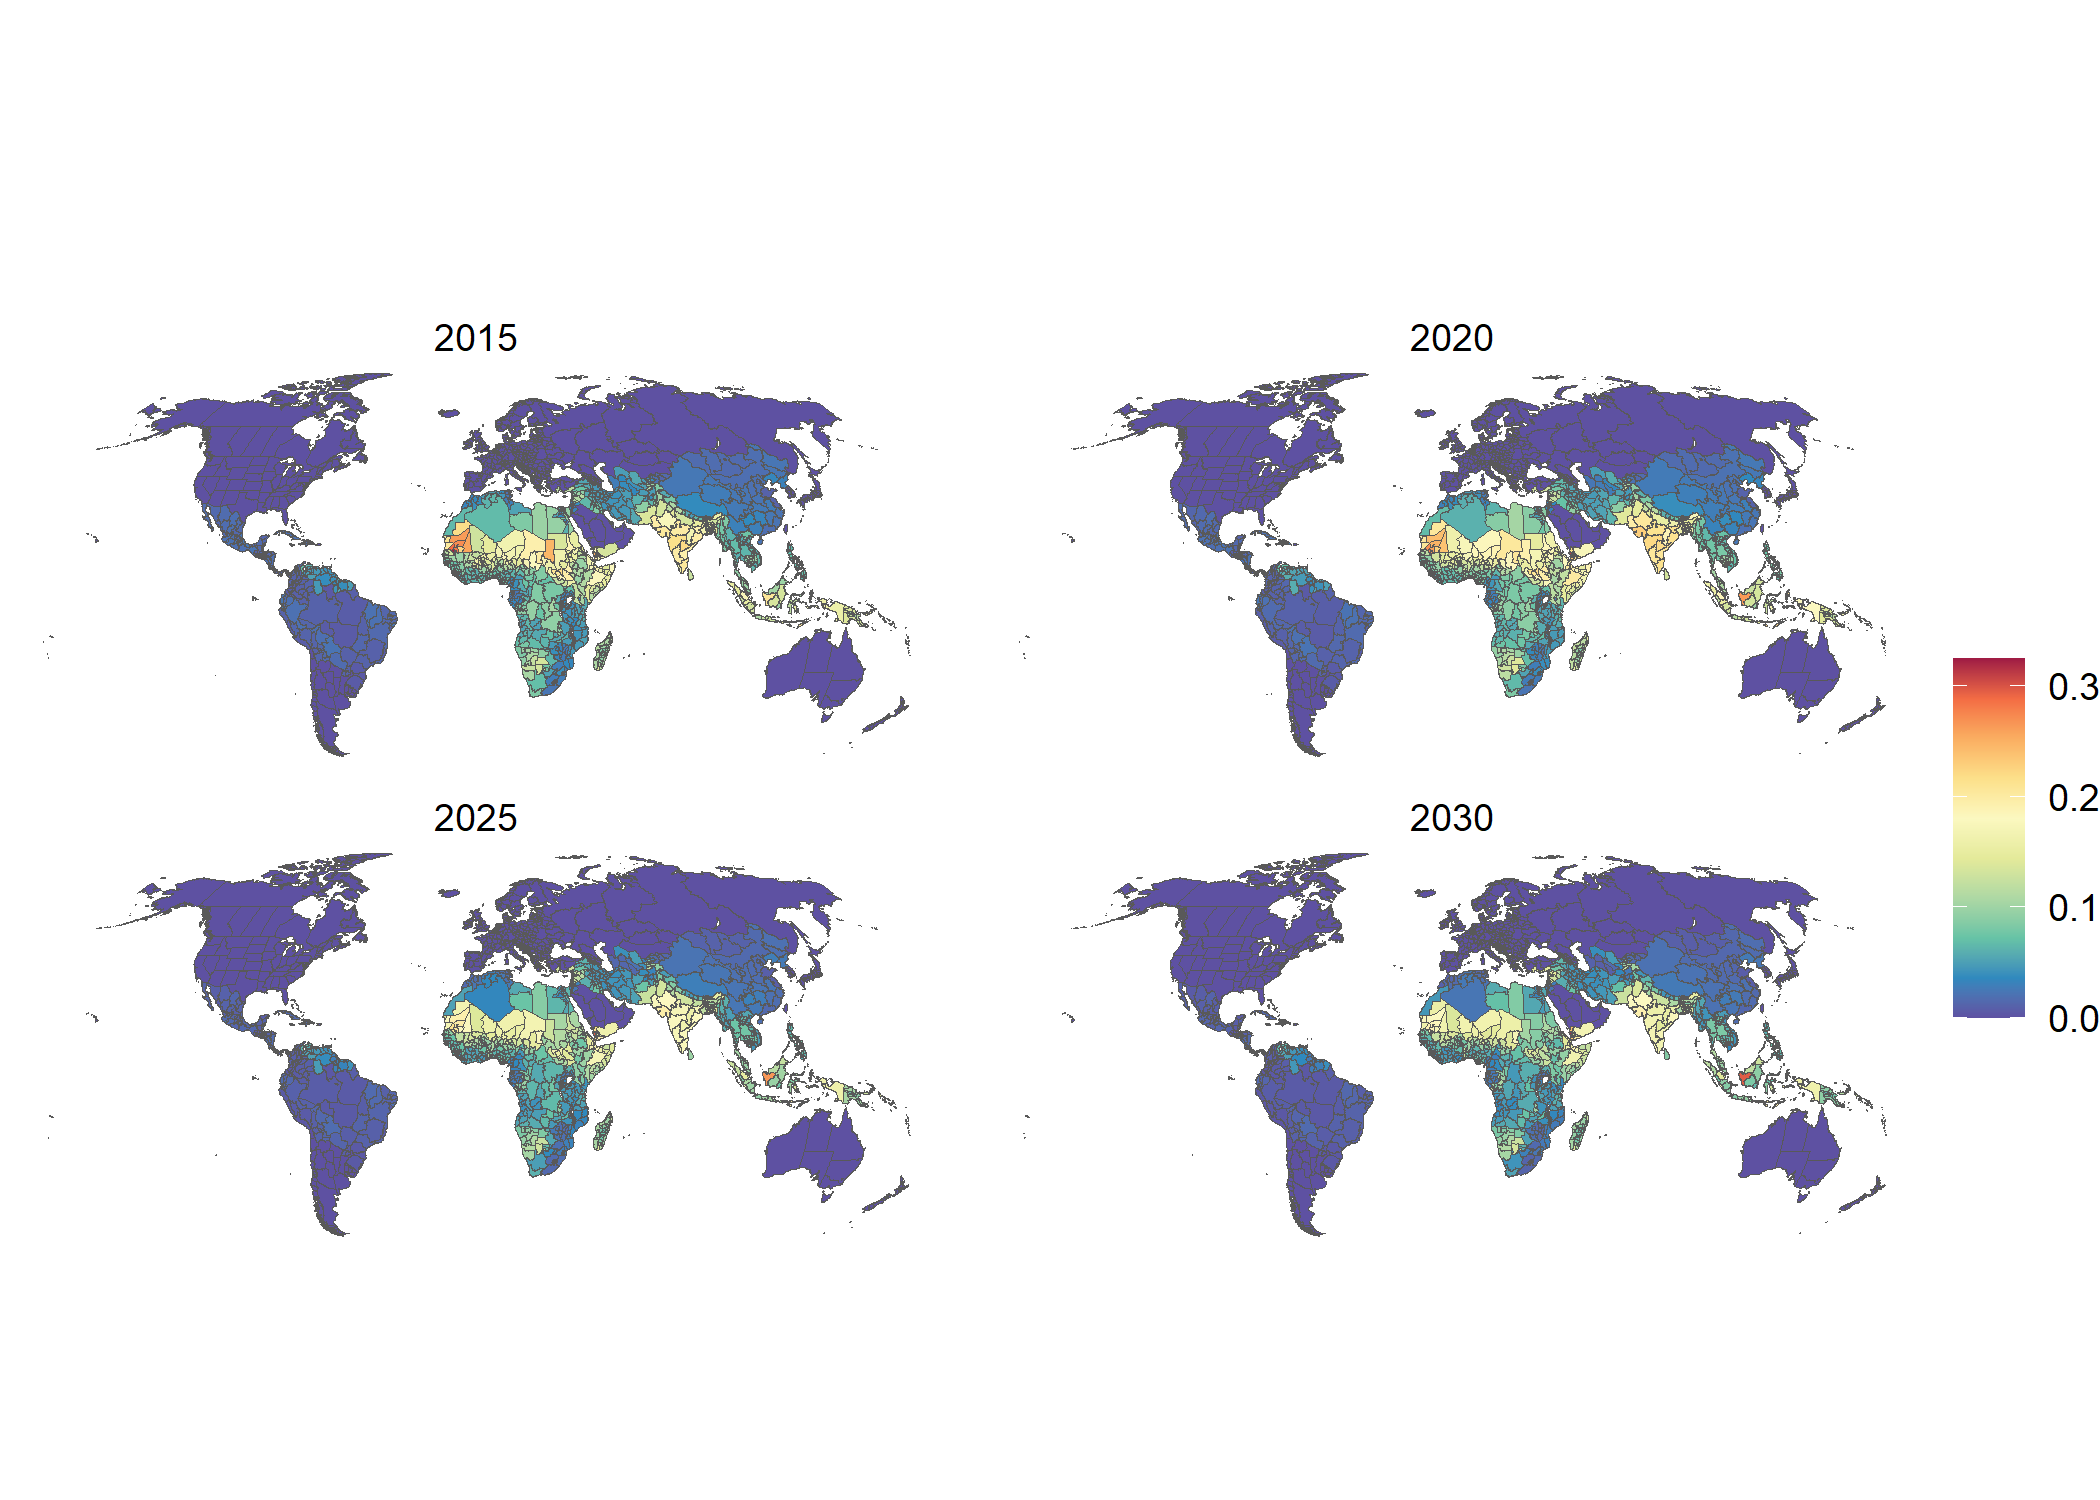
\includegraphics[width=\linewidth]{img/covars/wasting.png}
  \caption{Prevalence of wasting.}
\end{figure}

\subsection{Stunting}

We model stunting using the same methodology we use to summarize and model wasting, because the Local Burden of Disease dataset that we draw on for wasting also includes stunting.  We also included the 14.3\% increase in prevalence for the year 2020 that was estimated for wasting \citep{headey2020impacts}, even though stunting is a long-term consequence of malnutrition and will likely not be as readily observable in a population as wasting would be.  However, we use stunting in our model not as a cause of food insecurity, but rather as a proxy for chronic conditions of hunger, which are exacerbated by the coronavirus pandemic.  Thus, estimating an impact of the coronavirus shock on stunting is appropriate for our model.

\begin{figure}[H]
  \centering
  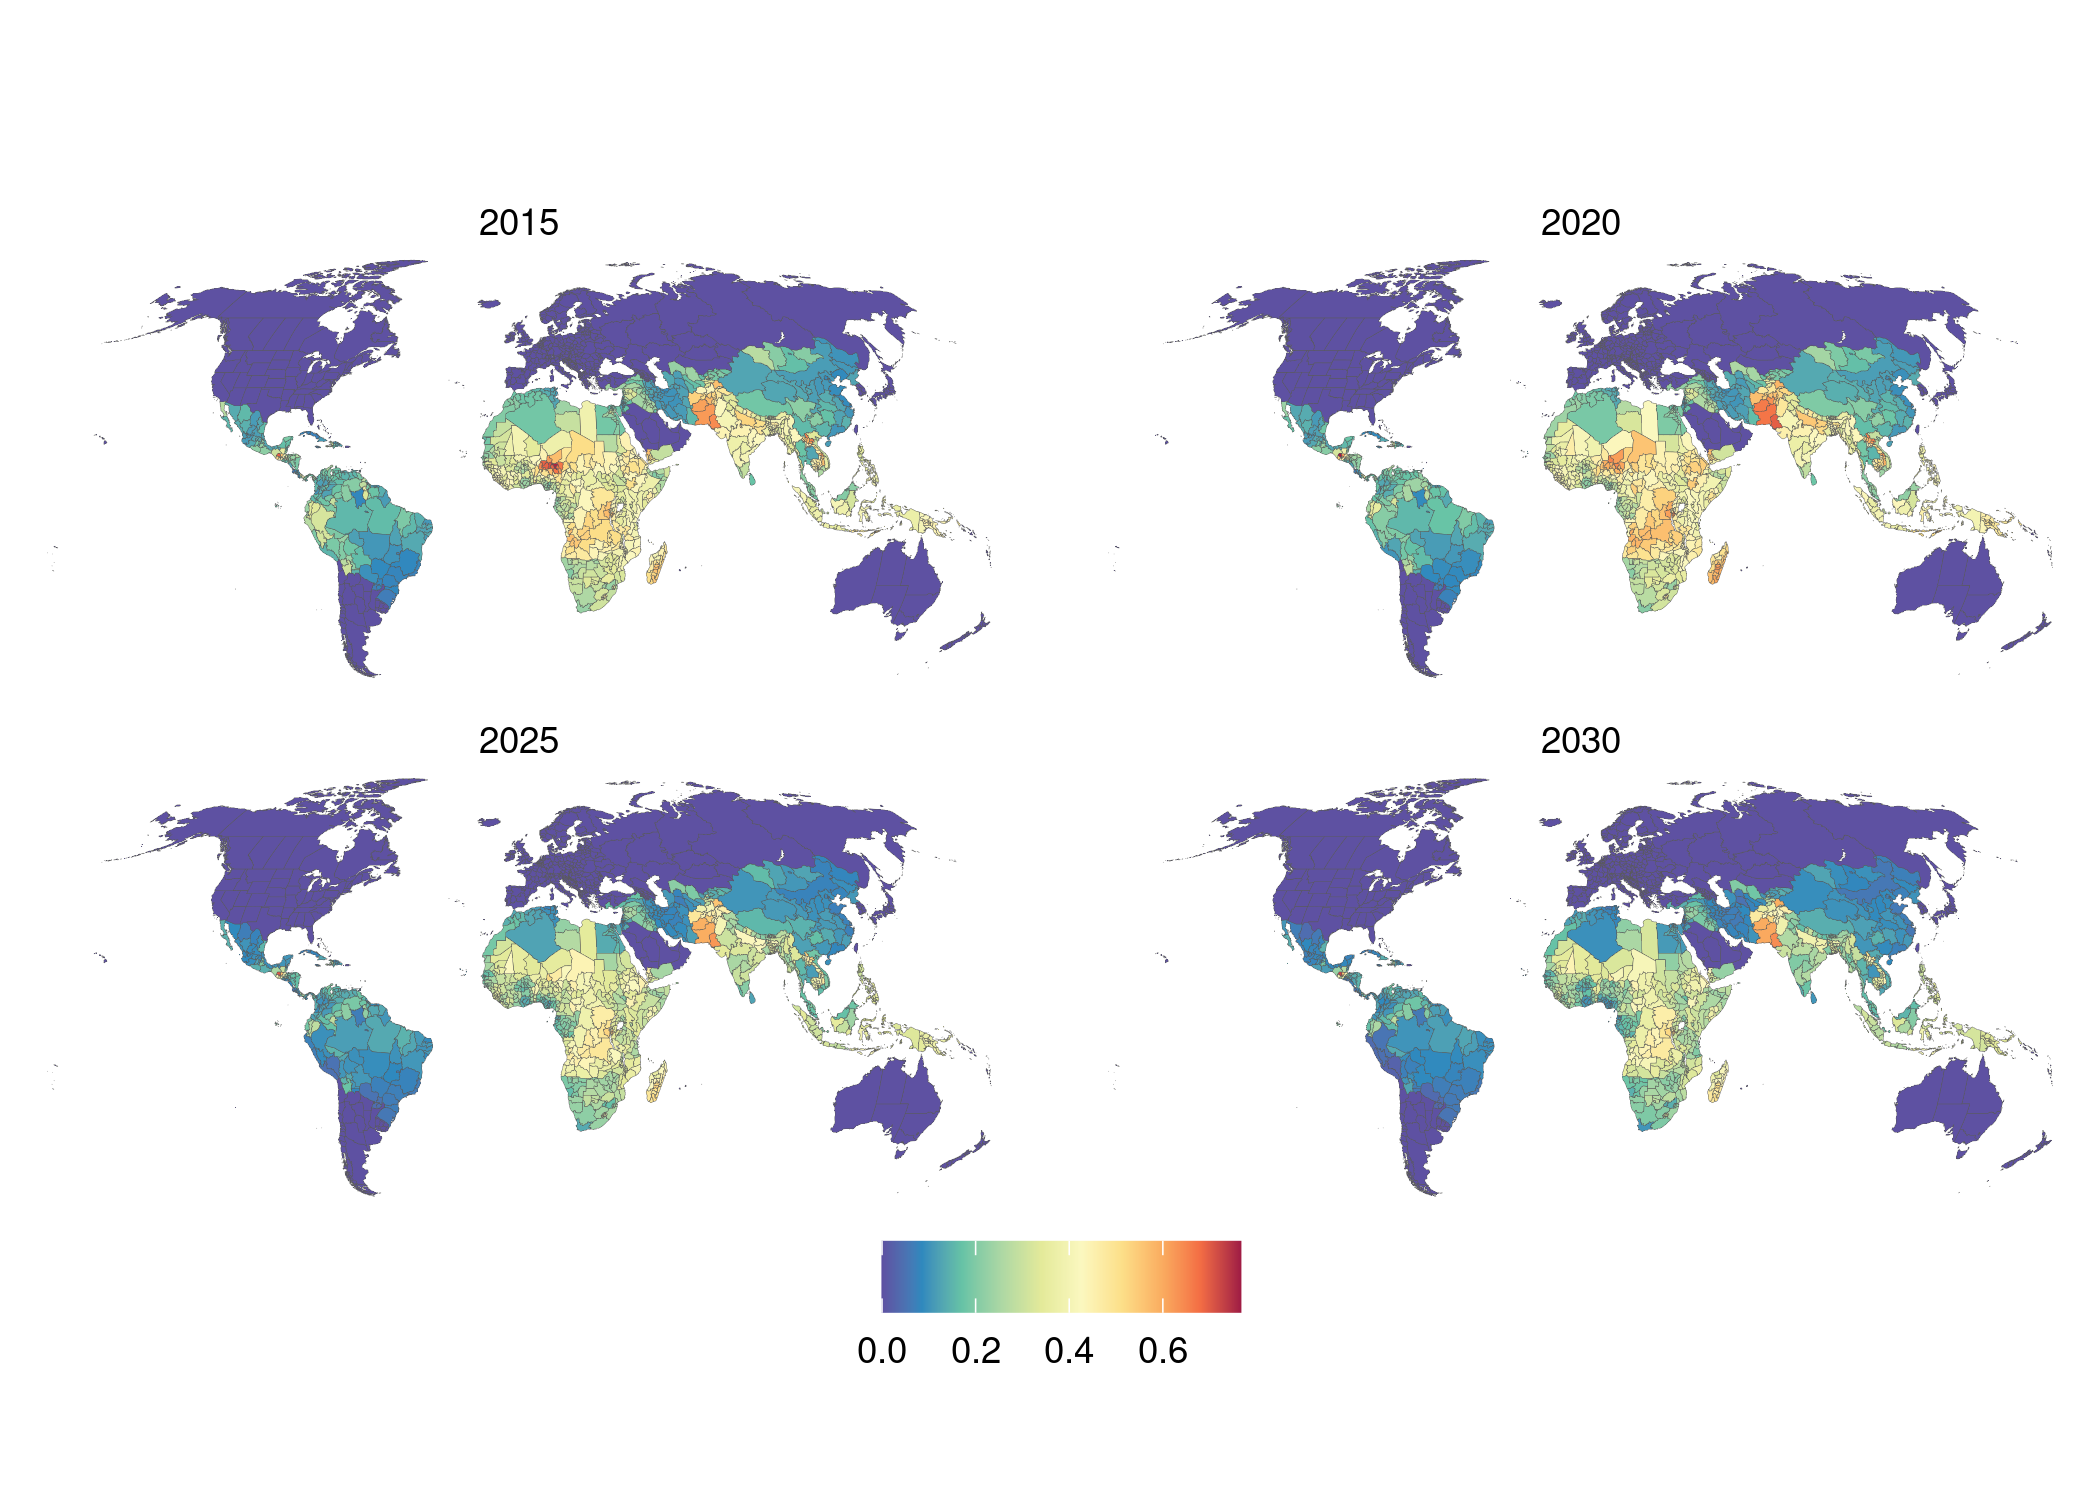
\includegraphics[width=\linewidth]{img/covars/stunting.png}
  \caption{Prevalence of stunting.}
\end{figure}

\subsection{GDP Per Capita}
We estimate global subnational GDP per capita using historic subnational estimates of Gross National Income (GNI) from the Subnational Human Development Database \cite{Smits2019} and forecasts of national GDP within the SSP framework from Dellink et al. \cite{Dellink2017}.  We first use data from the World Bank to estimate the mean country-level ratio of GNI to GDP and adjust the subnational estimates of GNI according to that country-specific ratio.  We then calculate each admin area's share of country GDP, and then use the AROC method to estimate each admin area's share of total country GDP.  Based on these trajectories in each admin areas share of total country GDP, we estimate what each admin area's share of GDP will be for each year from 2019 to 2030.  We divide that share of GDP by the population of the administrative area, which we had previously estimated.  Thus, national GDP totals are consistent with the projections of Dellink et al., but are disaggregated according to the historic patters of GDP share in the Subnational Human Development Database.

Finally, we used estimates of country-level changes in GDP growth for the years 2020 and 2021 to account for the impact of the coronavirus \citep{prospects2020}.  We then model GDP as resuming its previous growth trajectory based on previously-estimated growth rates from 2022-2030, but growing from an estimate for 2021 that includes the coronavirus shock.

\begin{figure}[H]
  \centering
  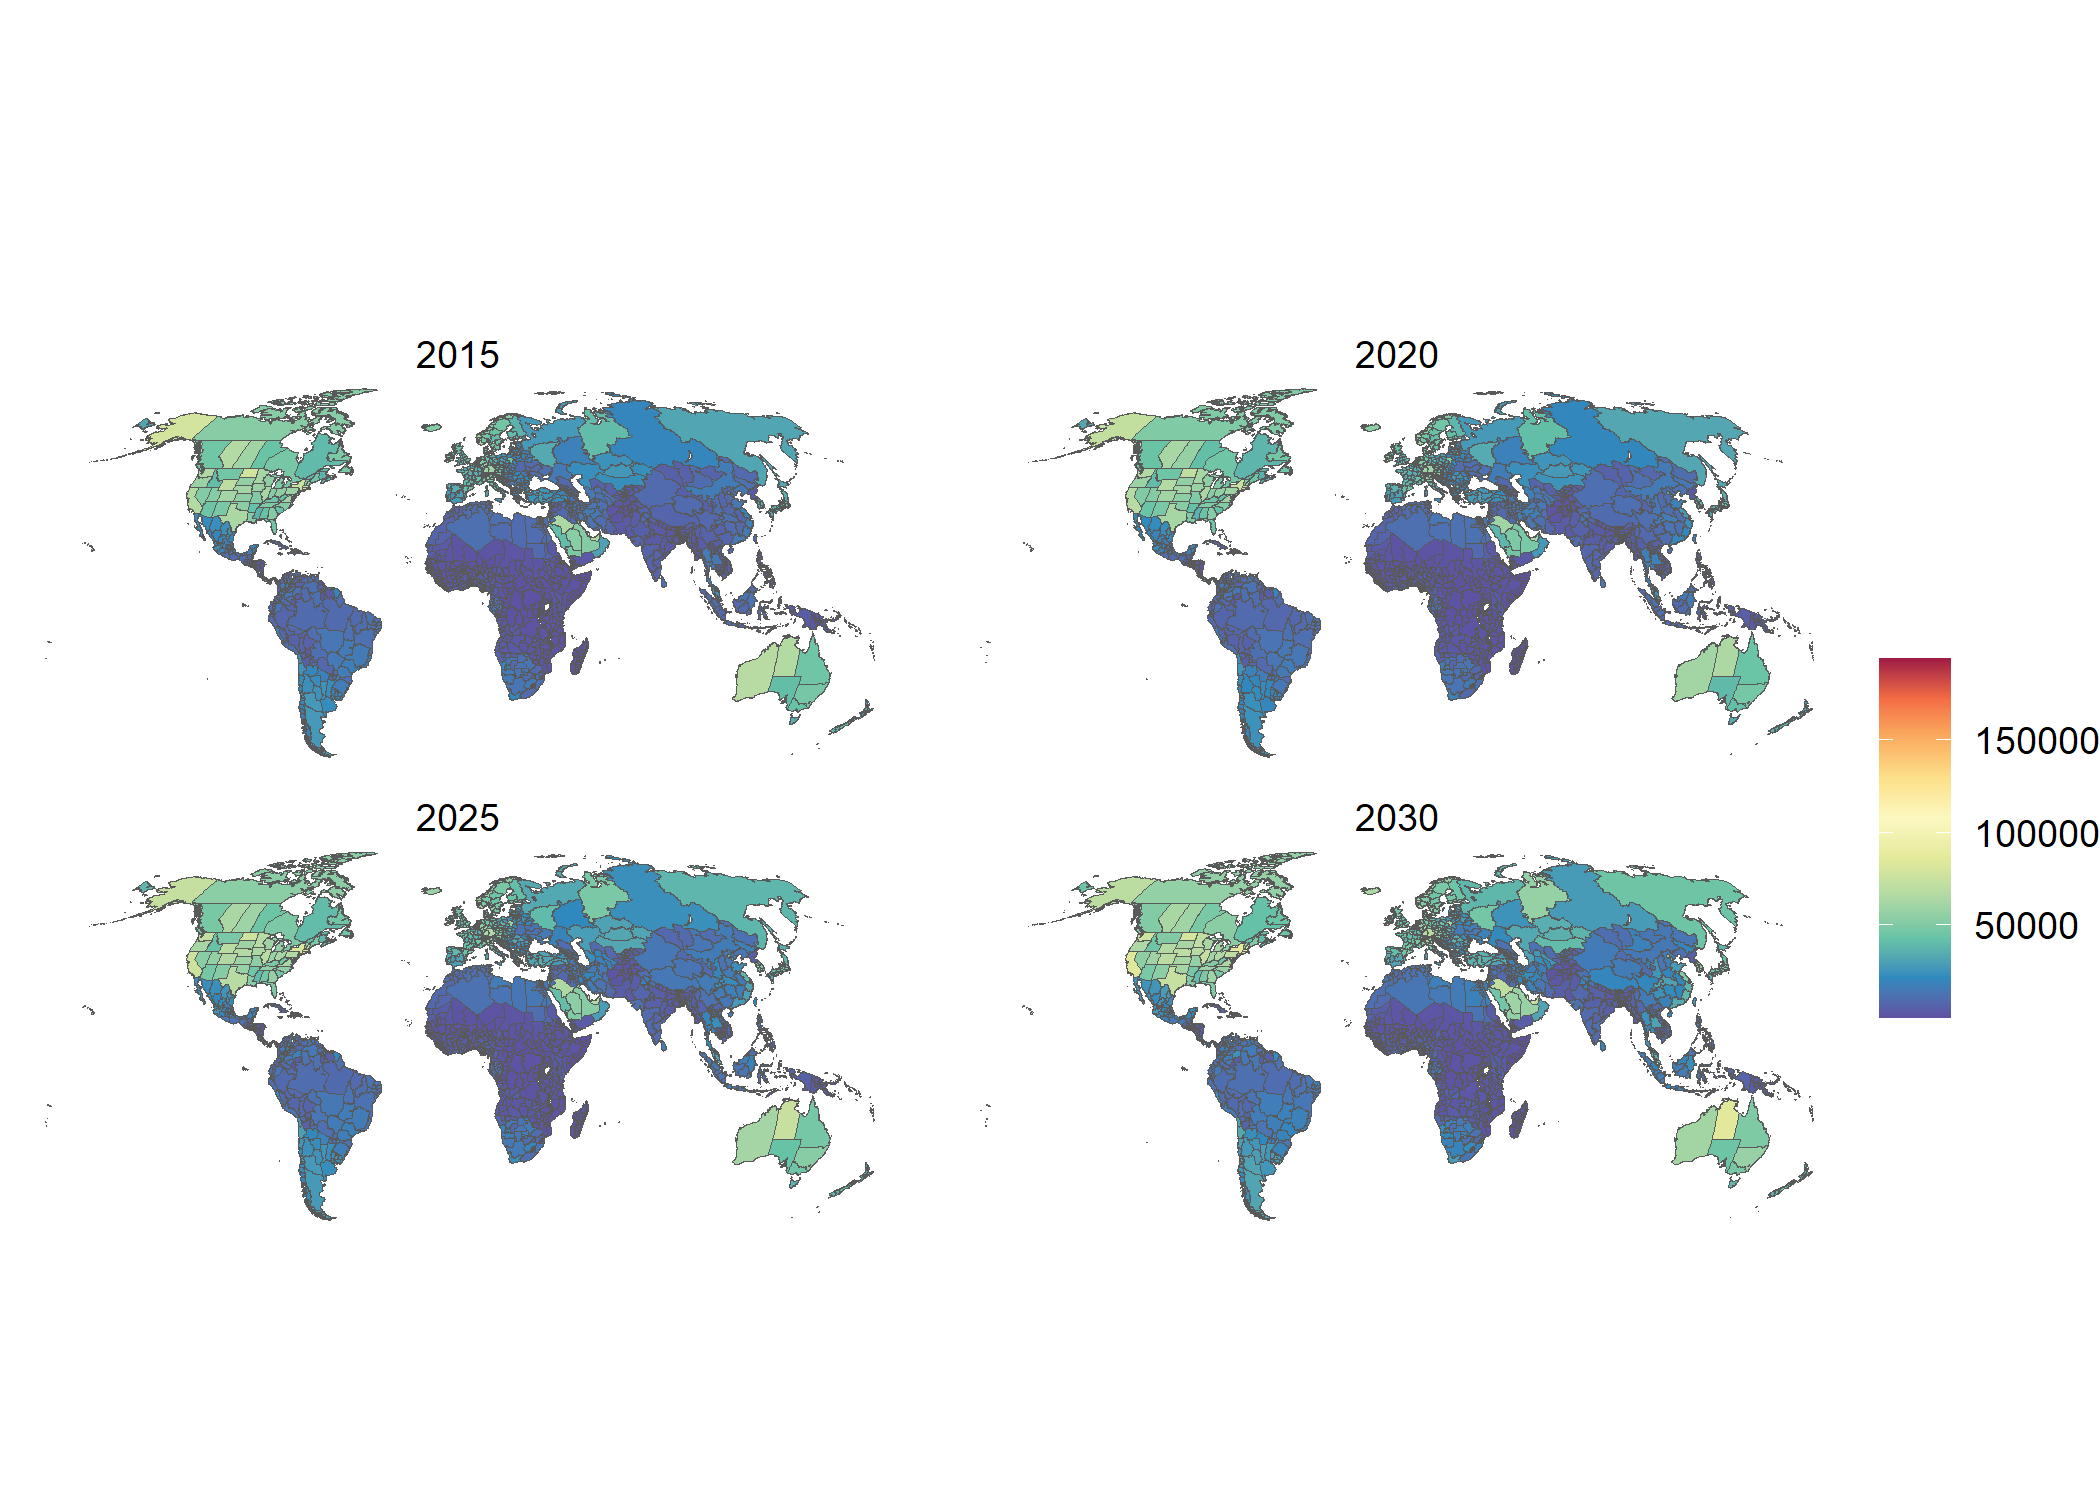
\includegraphics[width=\linewidth]{img/covars/gdp_percap.png}
  \caption{GDP per capita.}
\end{figure}

\subsection{Mean Years of Schooling}
We estimate global subnational mean years of schooling using historic subnational estimates from the Subnational Human Development Database \cite{Smits2019} and forecasts of national mean years of schooling from KC et al. \cite{KC2017}.  Using the historic subnational data, we estimate each subnational administrative area's difference in years of schooling from the national mean, and use this value to disaggregate the future projections to a subnational level.


\begin{figure}[H]
  \centering
  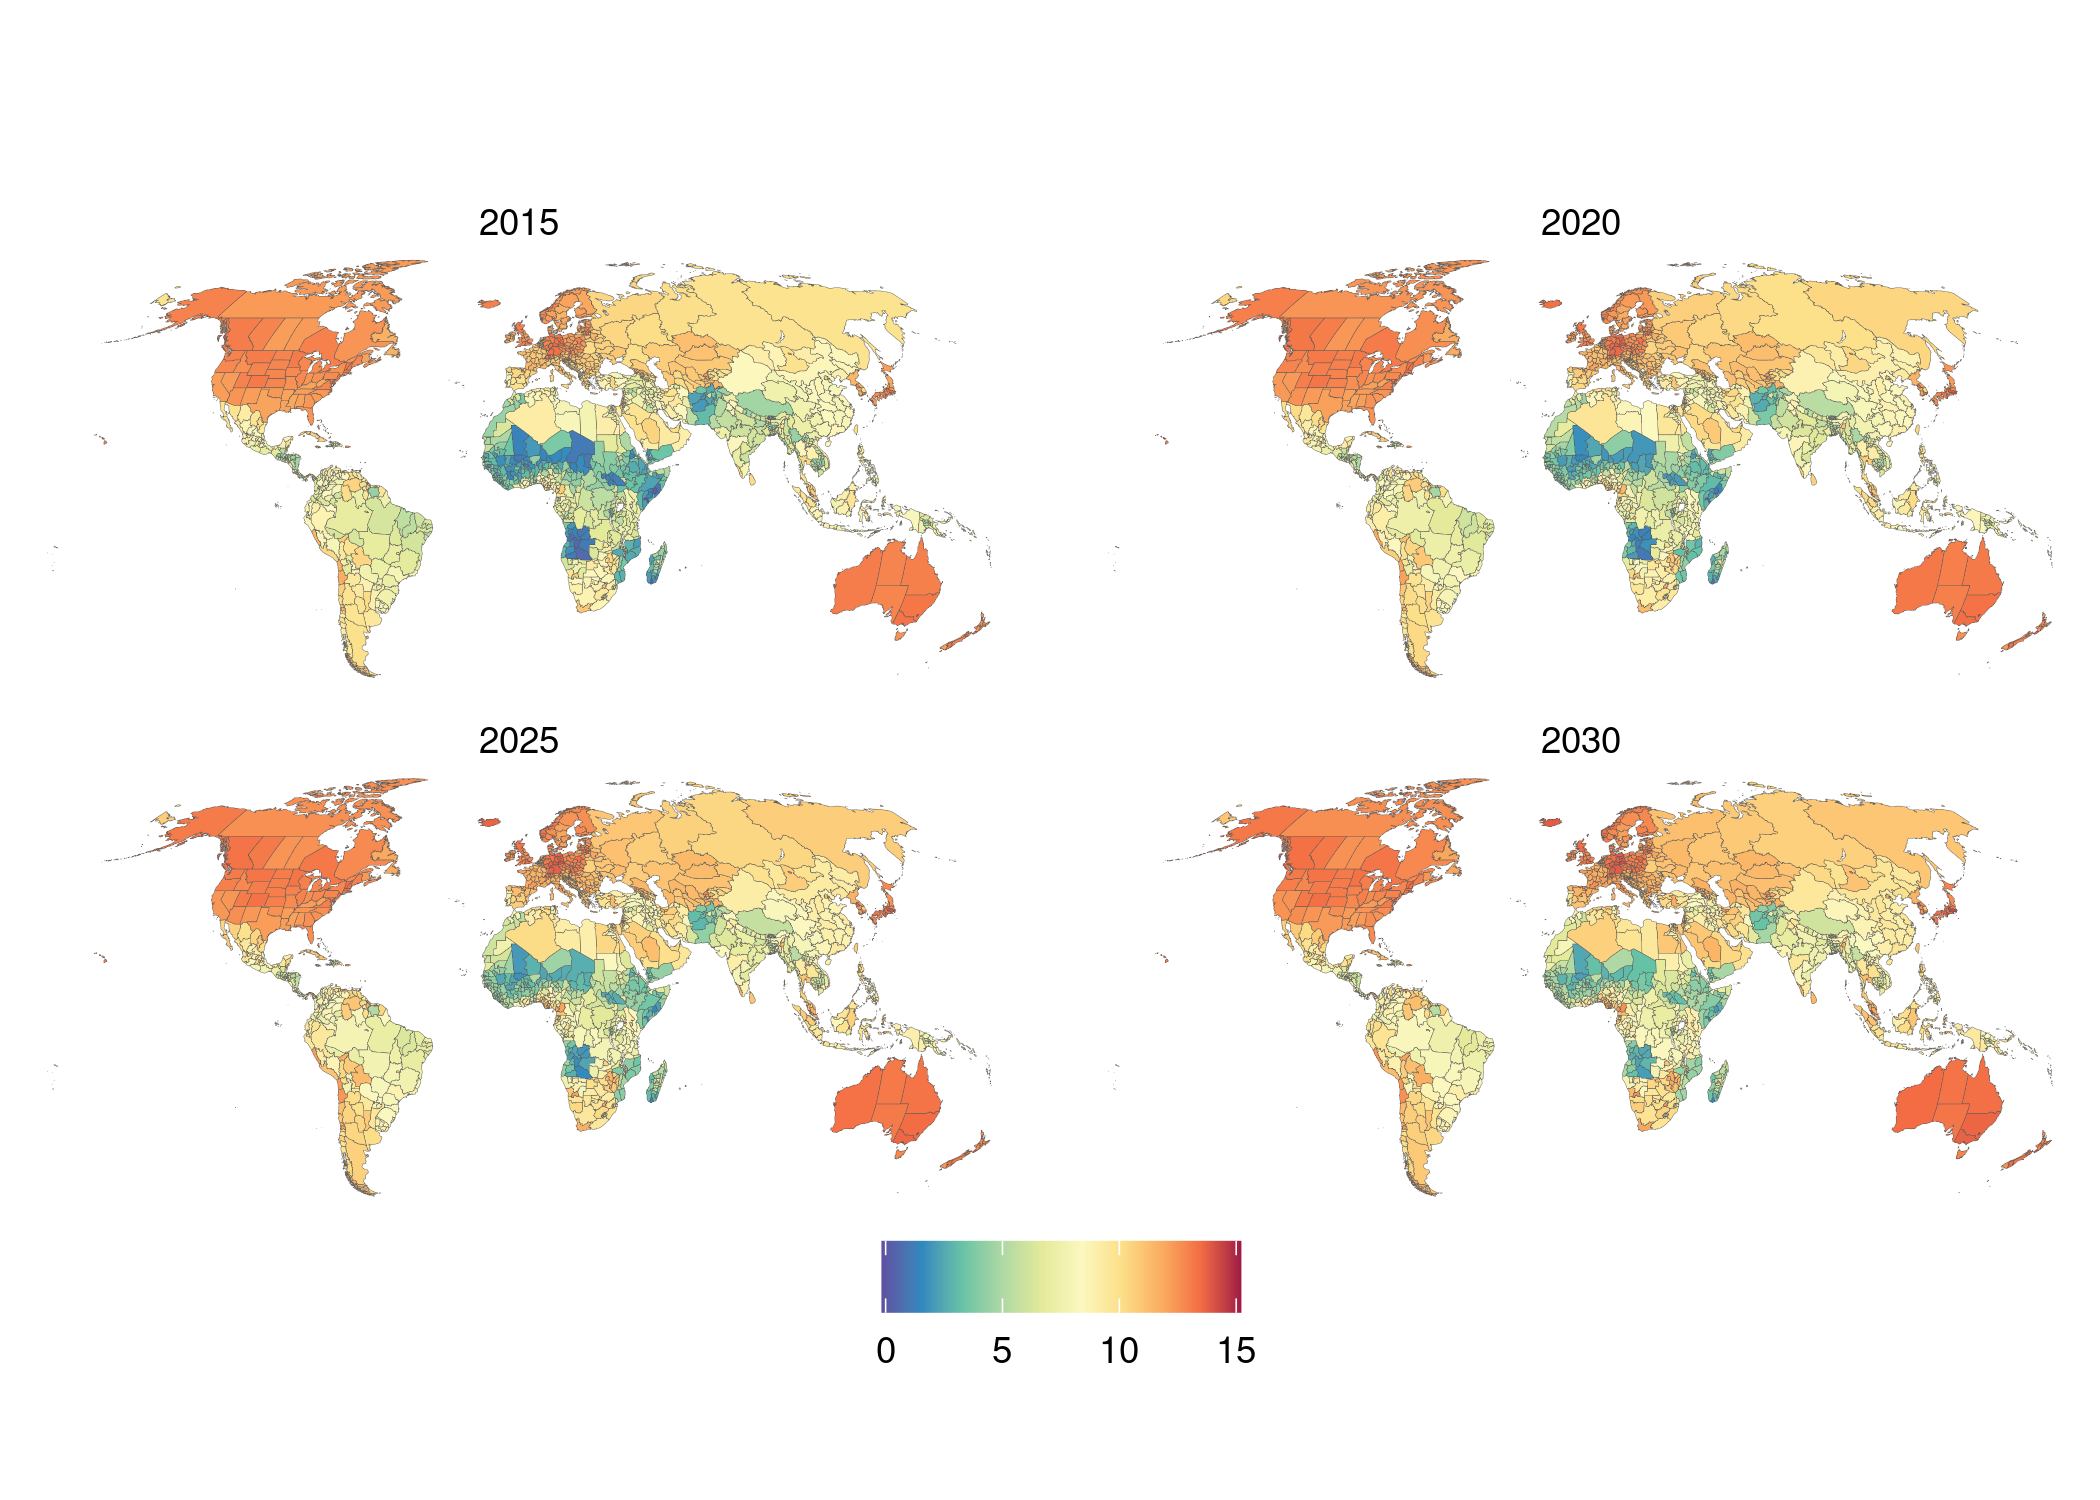
\includegraphics[width=\linewidth]{img/covars/school_mean.png}
  \caption{Mean years of schooling.}
\end{figure}


\subsection{Gini Coefficient}
We use estimates of national income inequality from Rao et al. \citep{Rao2019a}.  These estimates include all years in our analysis, and are not disaggregated to a subnational level.

\begin{figure}[H]
  \centering
  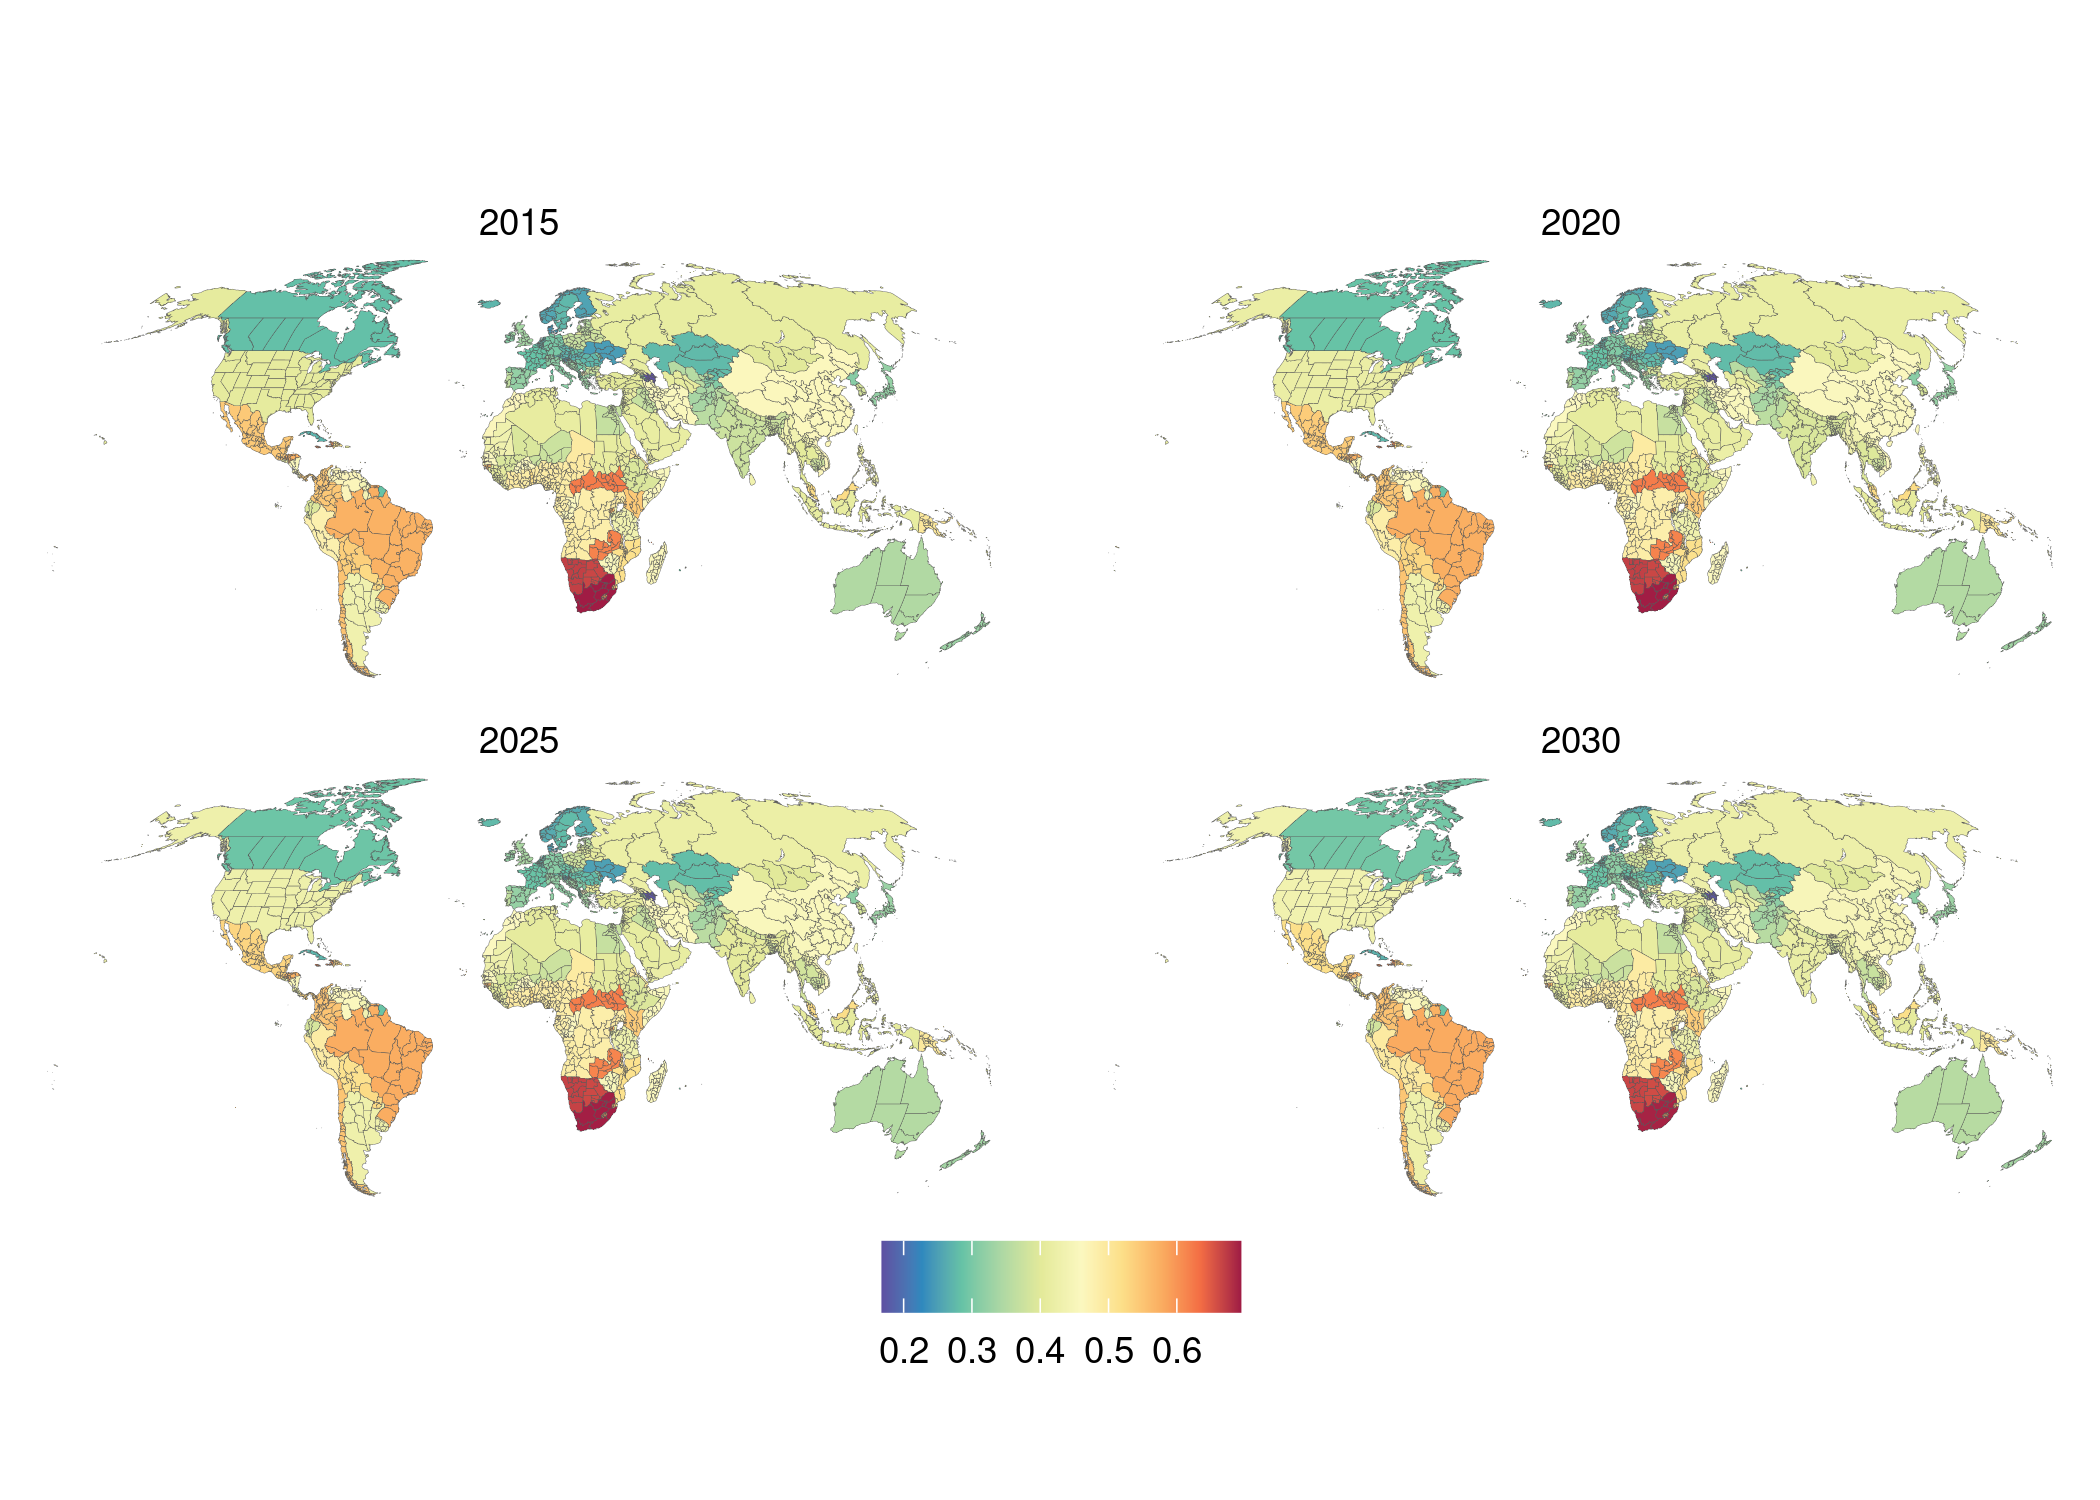
\includegraphics[width=\linewidth]{img/covars/gini.png}
  \caption{Gini Coefficient}
\end{figure}

\subsection{Poverty Headcount Index}
We used estimates of the Poverty Headcount Index for the recent past and future from the World Poverty Clock by the World Data Lab \citep{cuaresma2018will}, updated to include the impact of the coronavirus. In our model we include national level poverty rates at a threshold of \$1.90 which is defined as \textit{extreme} poverty. By using the concept of parameterized Lorenz curves in combination with mean income/consumption and population projections future poverty rates are calculated. For more details on the methodology and information on global and country level poverty check the website \url{worldpoverty.io}.

\begin{figure}[H]
  \centering
  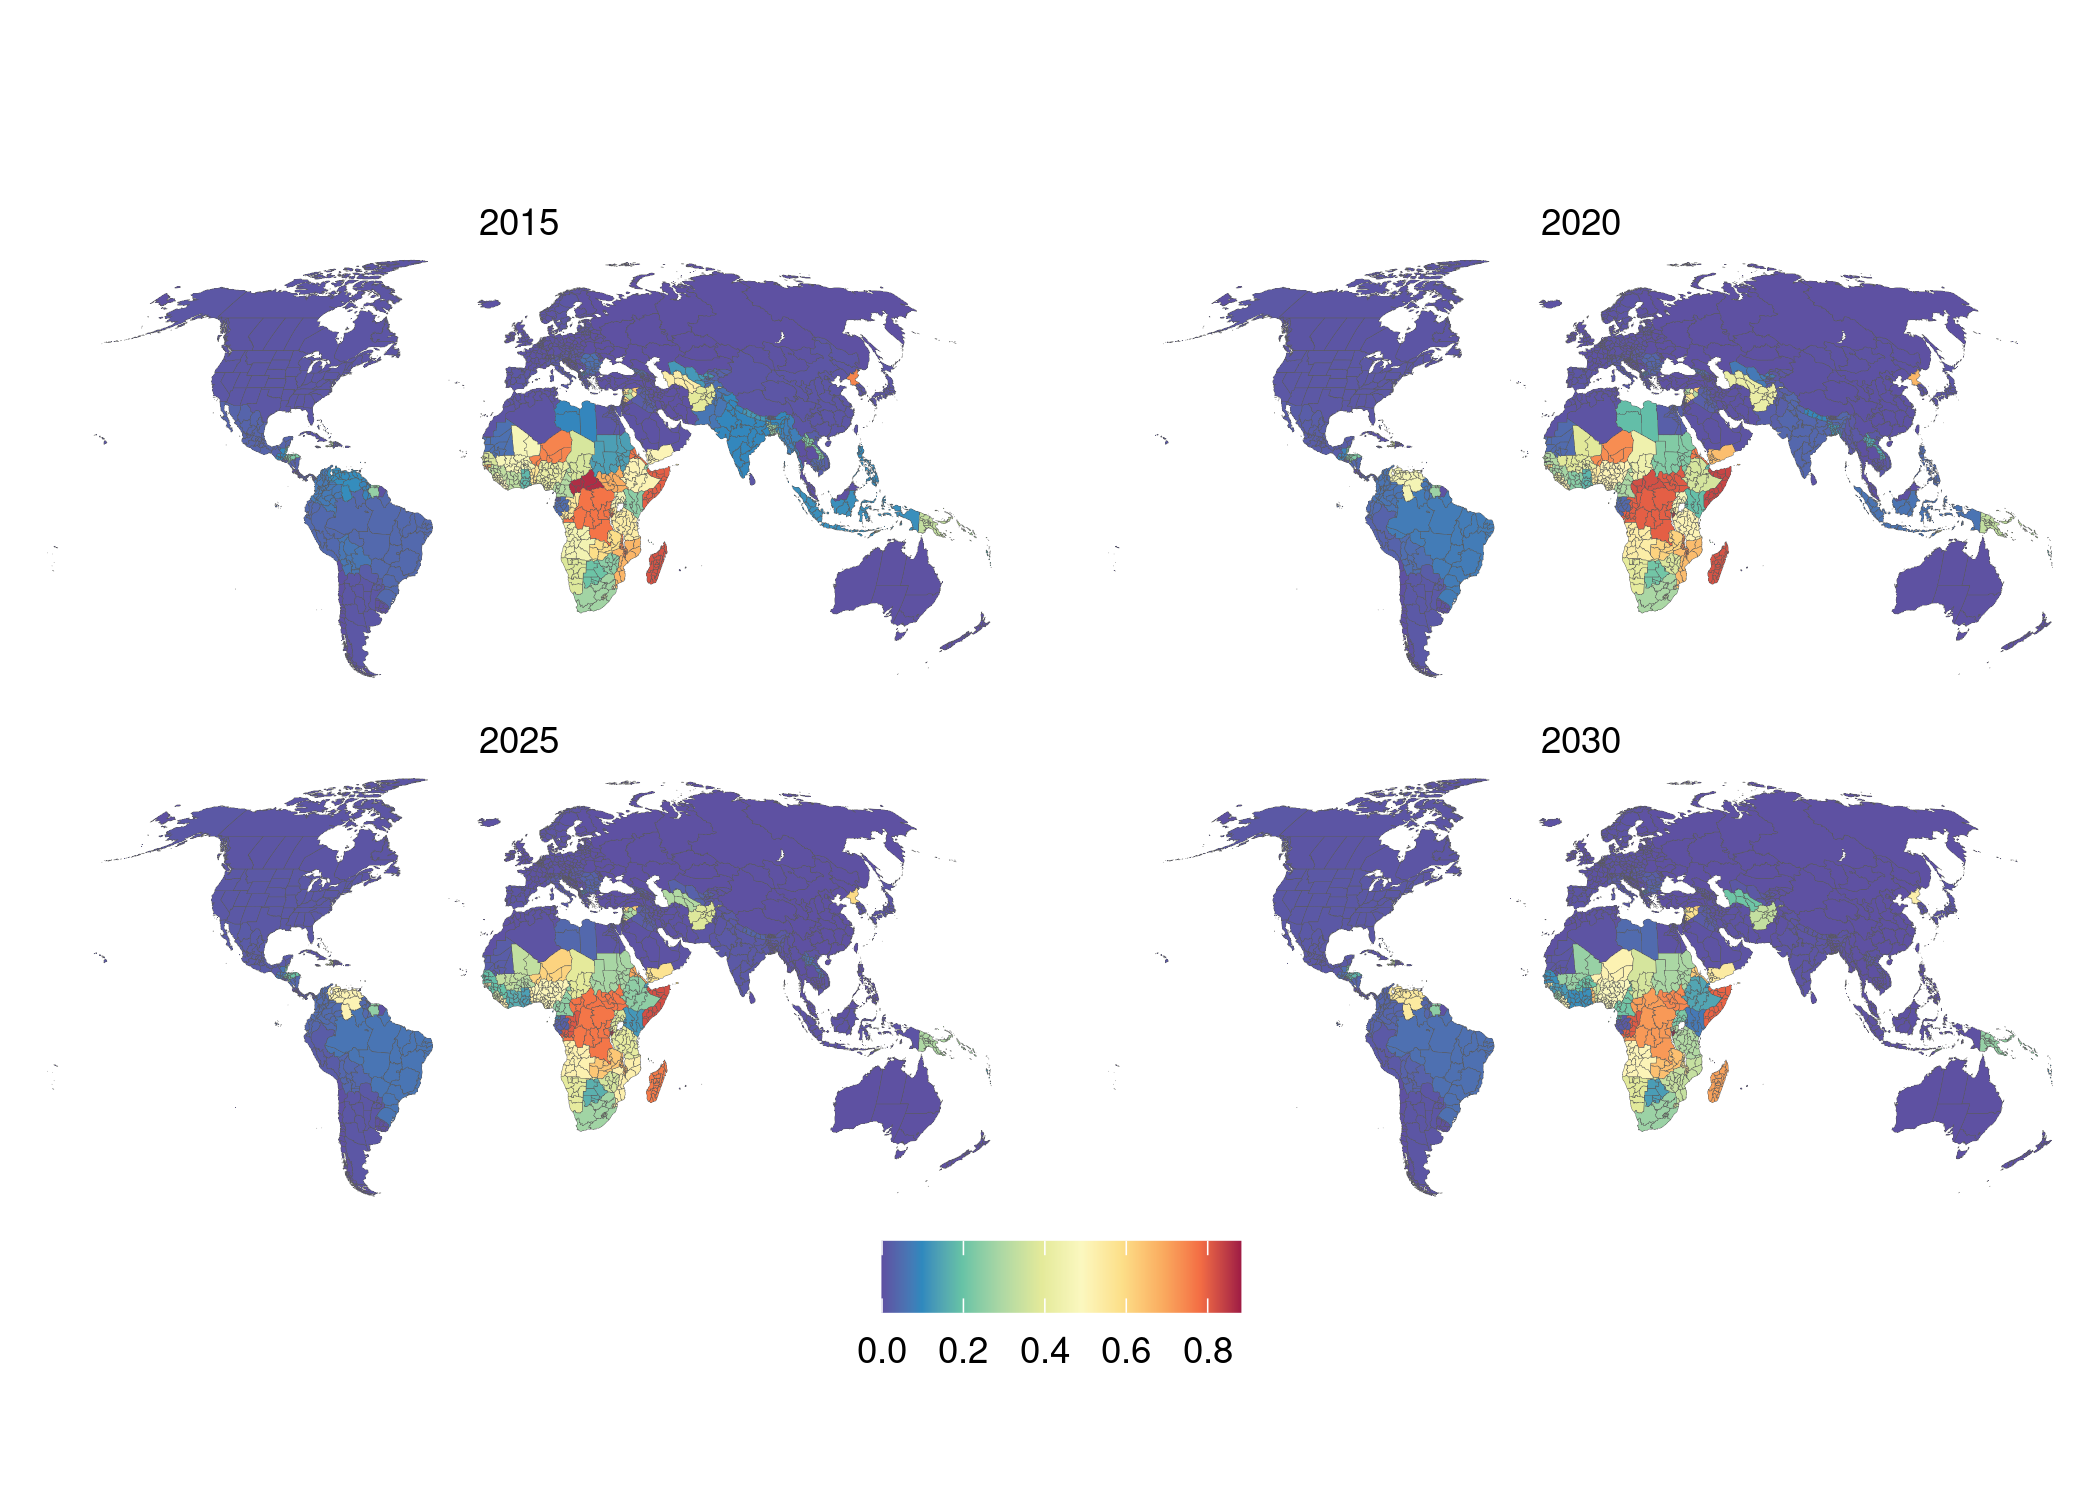
\includegraphics[width=\linewidth]{img/covars/hci.png}
  \caption{Poverty Headcount Index}
\end{figure}


\subsection{Water Scarcity}
\begin{figure}[H]
  \centering
  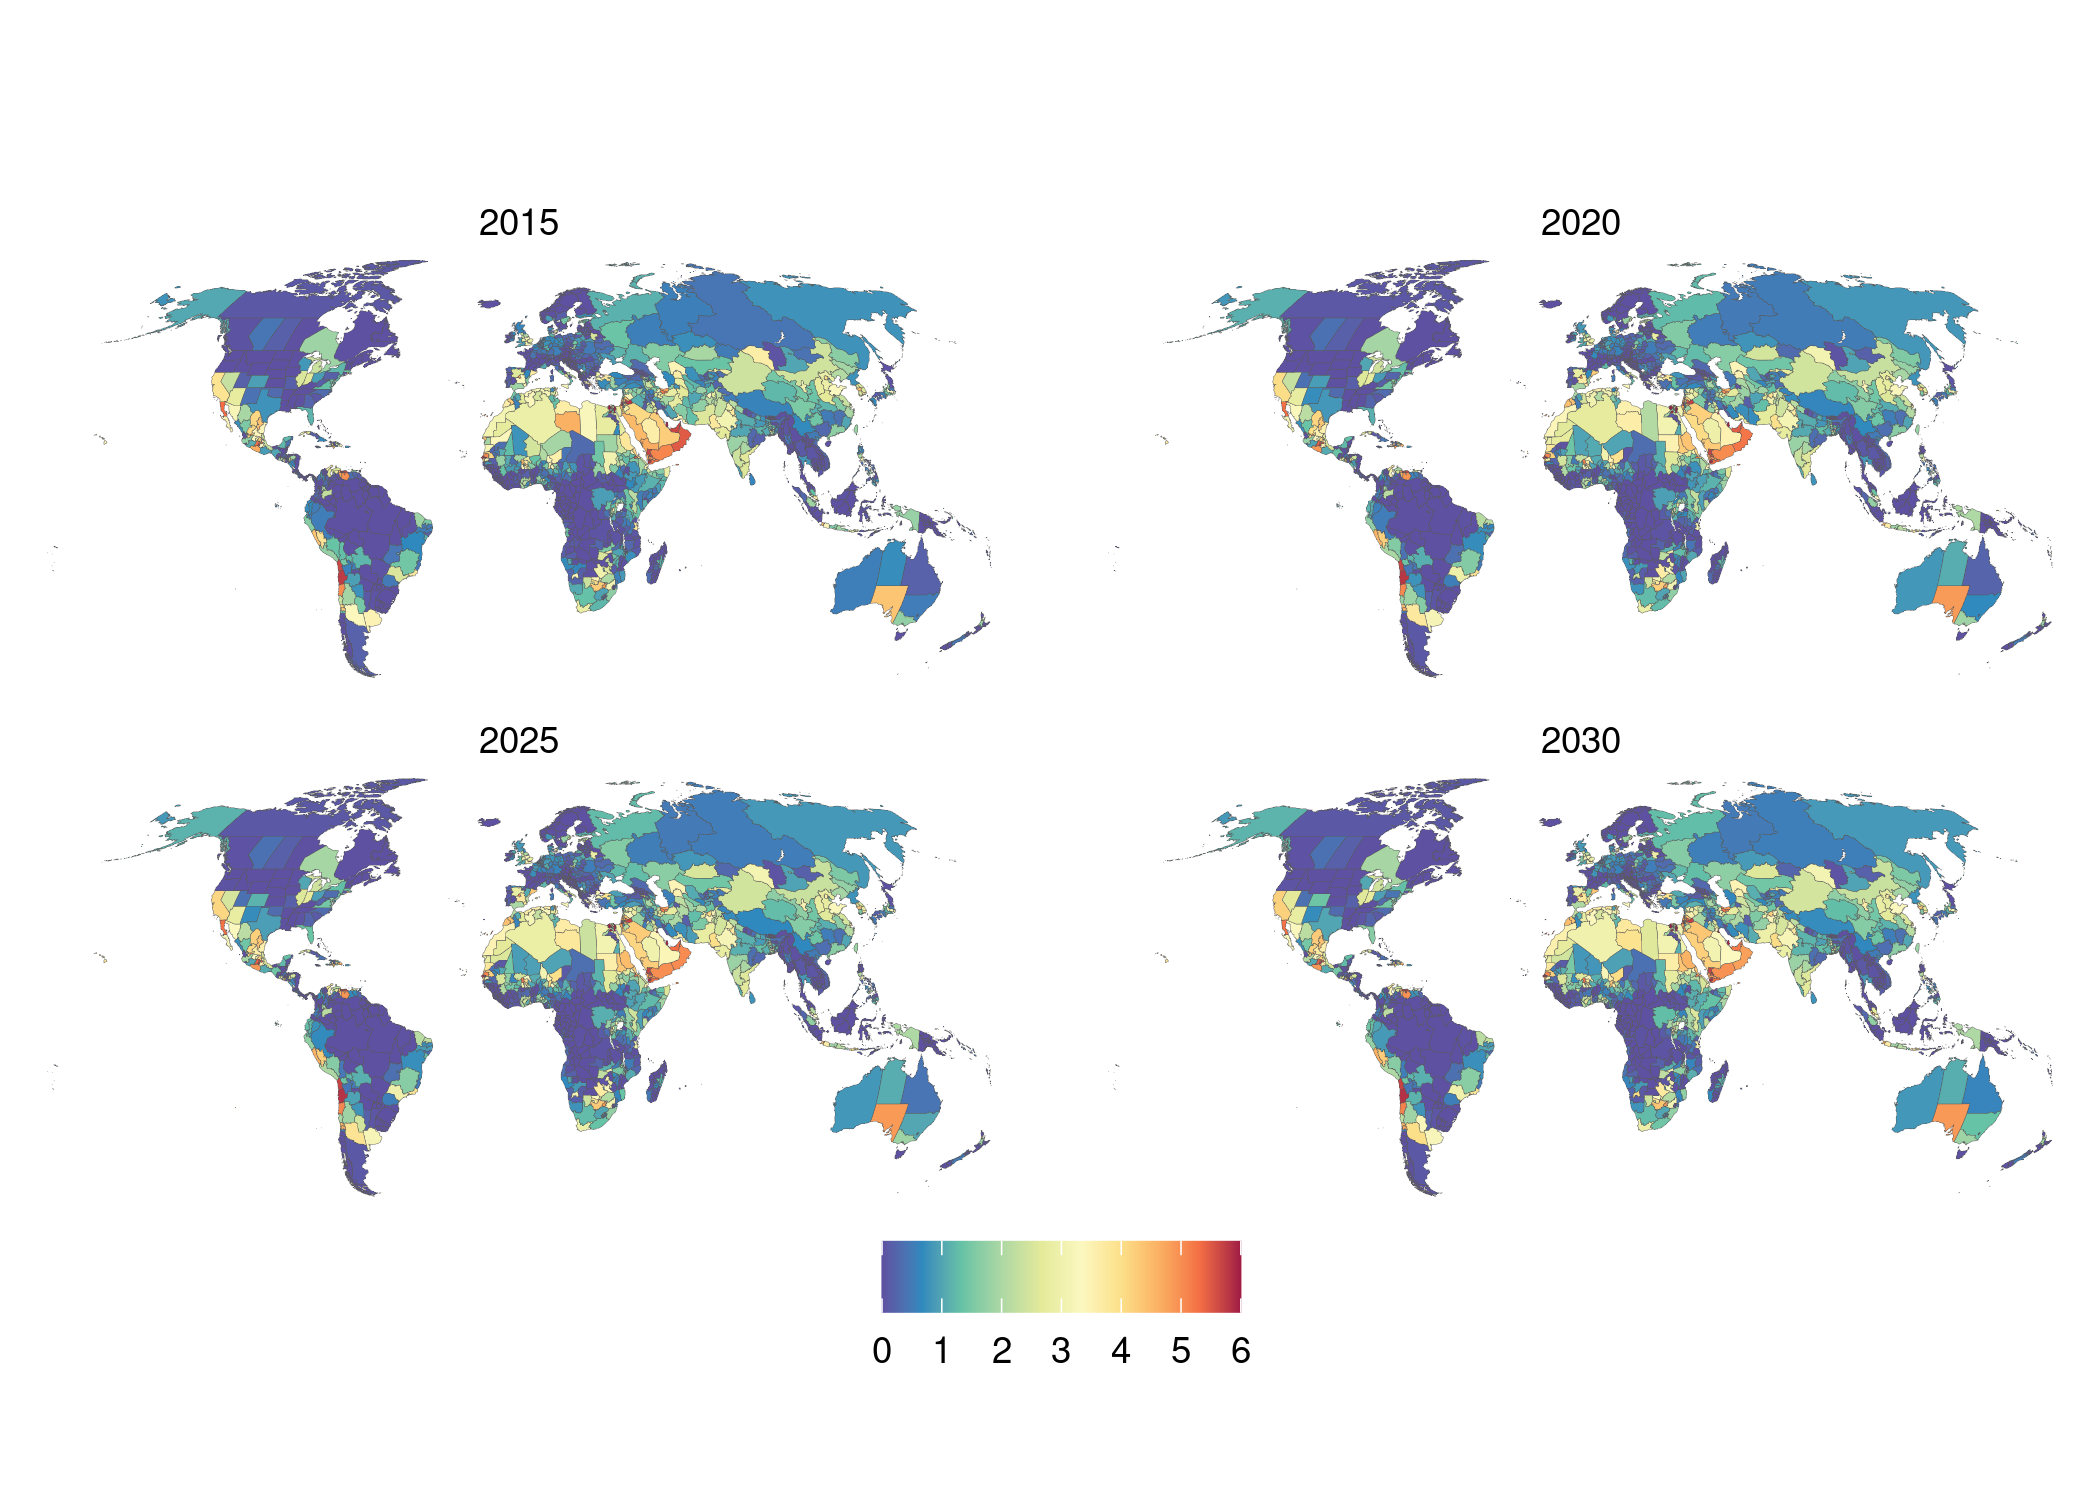
\includegraphics[width=\linewidth]{img/covars/wci_index.png}
  \caption{Water Scarcity Index}
\end{figure}


\subsection{Mean Annual Precipitation}
For mean annual precipitation, we use data for the years 2010 to 2019 from the TerraClimate dataset \citep{abatzoglou2018terraclimate}, summarized to each admin area.  For data for the years 2020-2030, we use models from the Inter-Sectoral Model Intercomparison Project \citep{warszawski2014inter}.  Specifically, we use an ensemble of bias-corrected projections under representative concentration pathway (RCP) 6.0, taking the mean of the ensemble.

\begin{figure}[H]
  \centering
  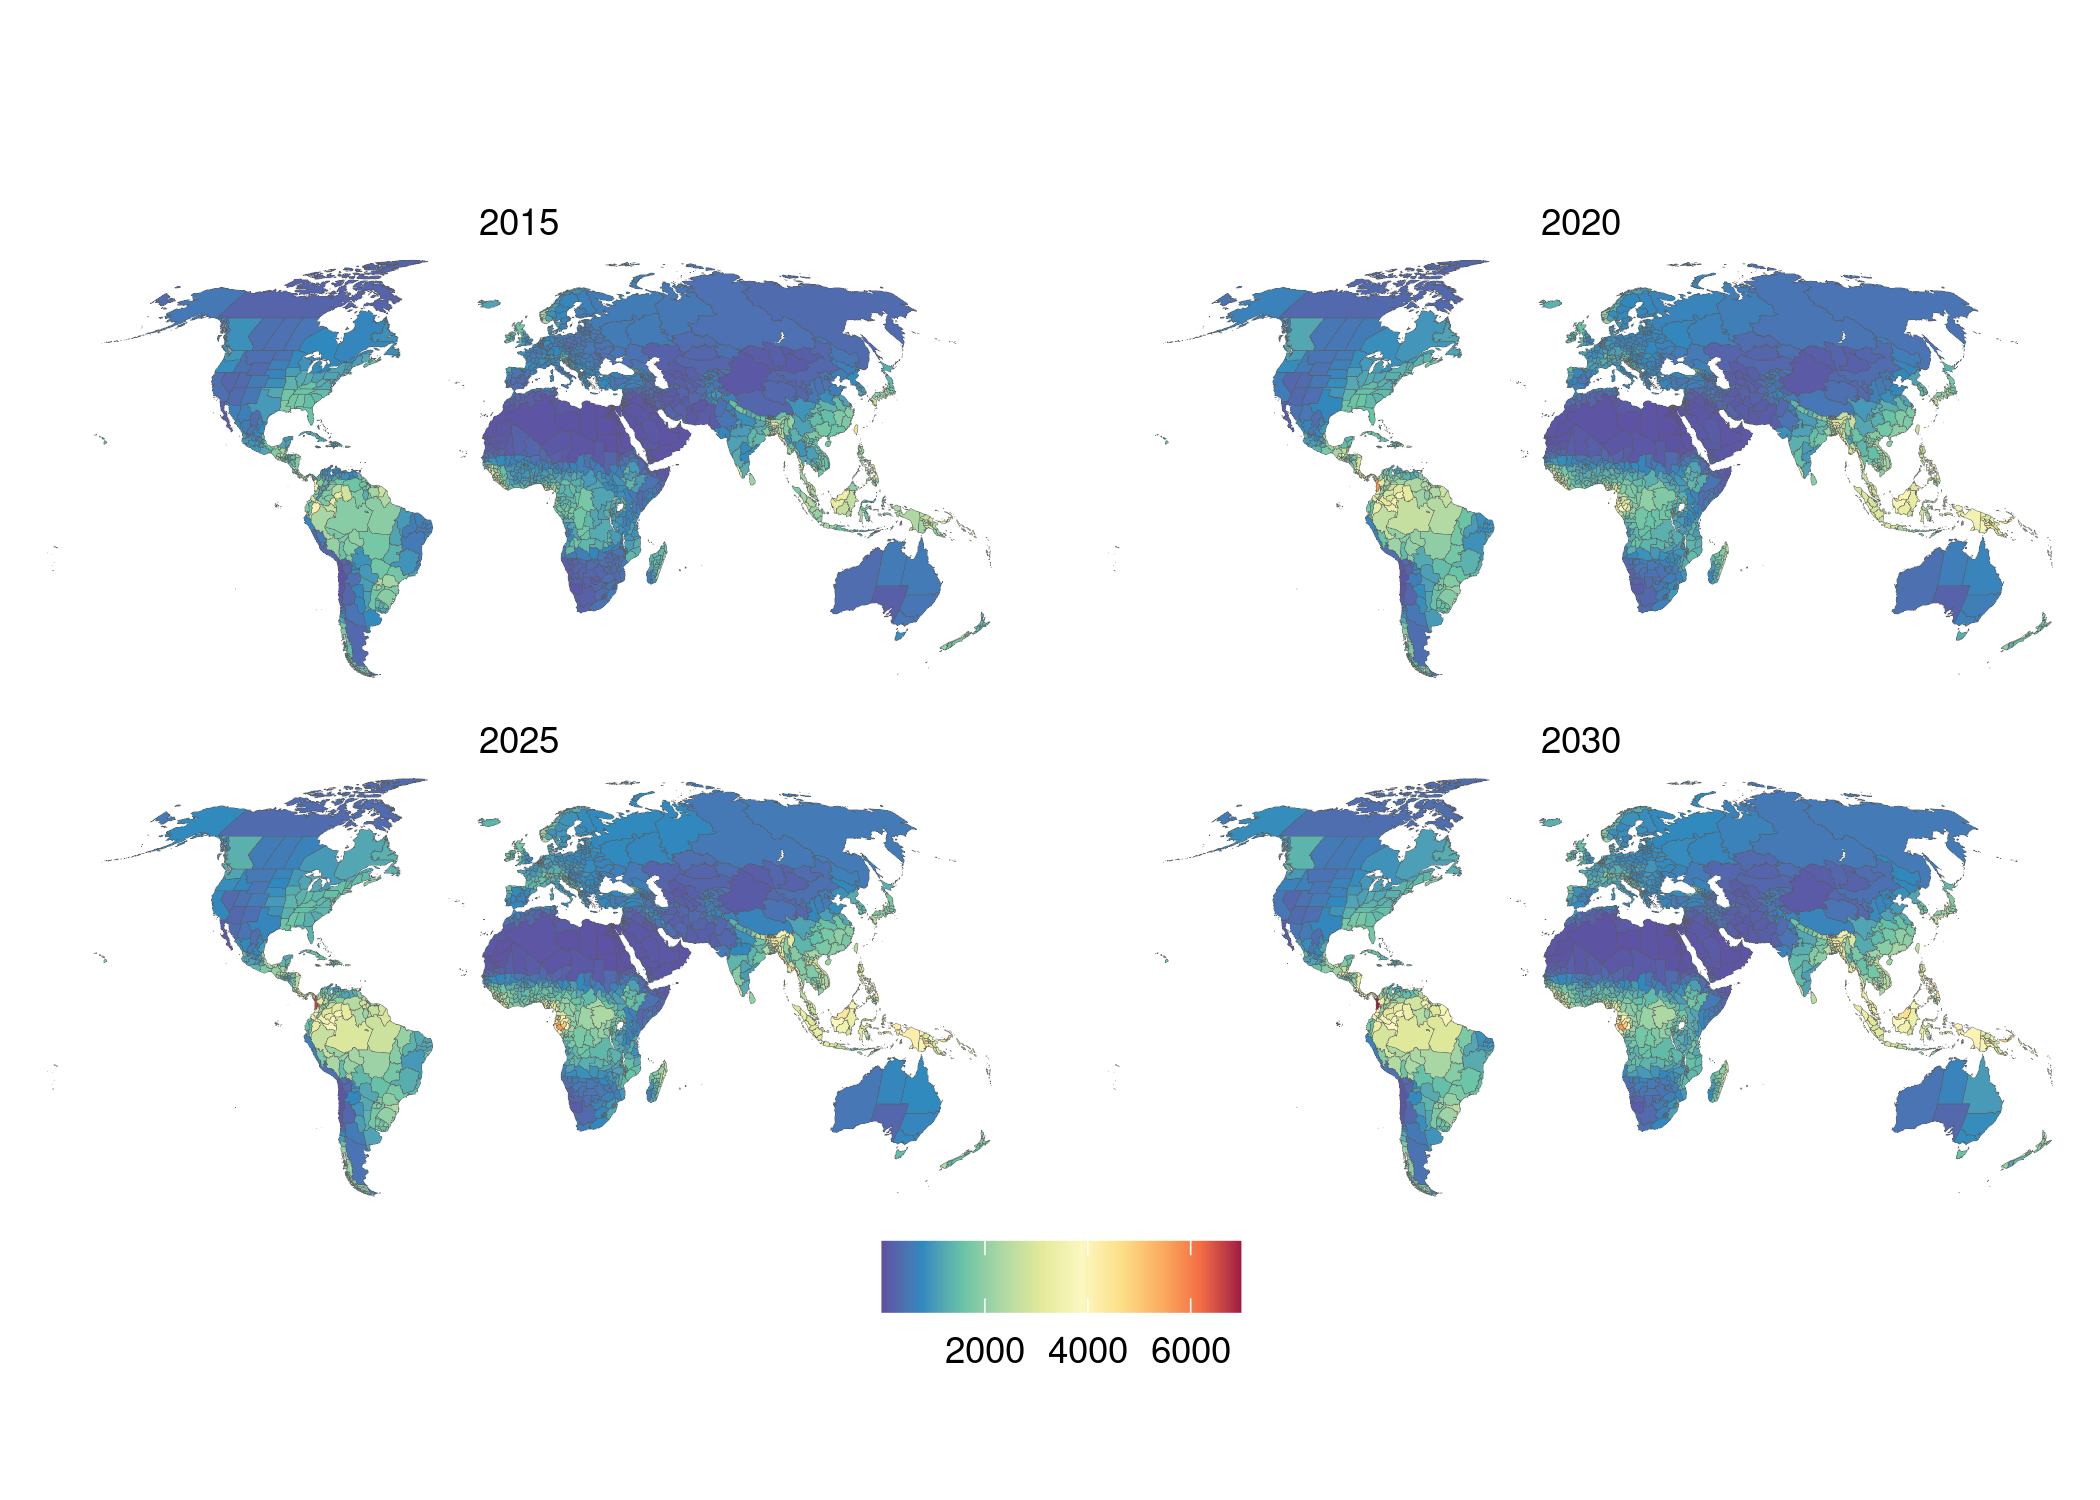
\includegraphics[width=\linewidth]{img/covars/precip.png}
  \caption{Mean annual precipitation}
\end{figure}

\subsection{Mean Temperature}
For mean temperature, we used the same datasets that we'd used for precipitation, as each of those datasets included both temperature in addition to precipitation.

\begin{figure}[H]
  \centering
  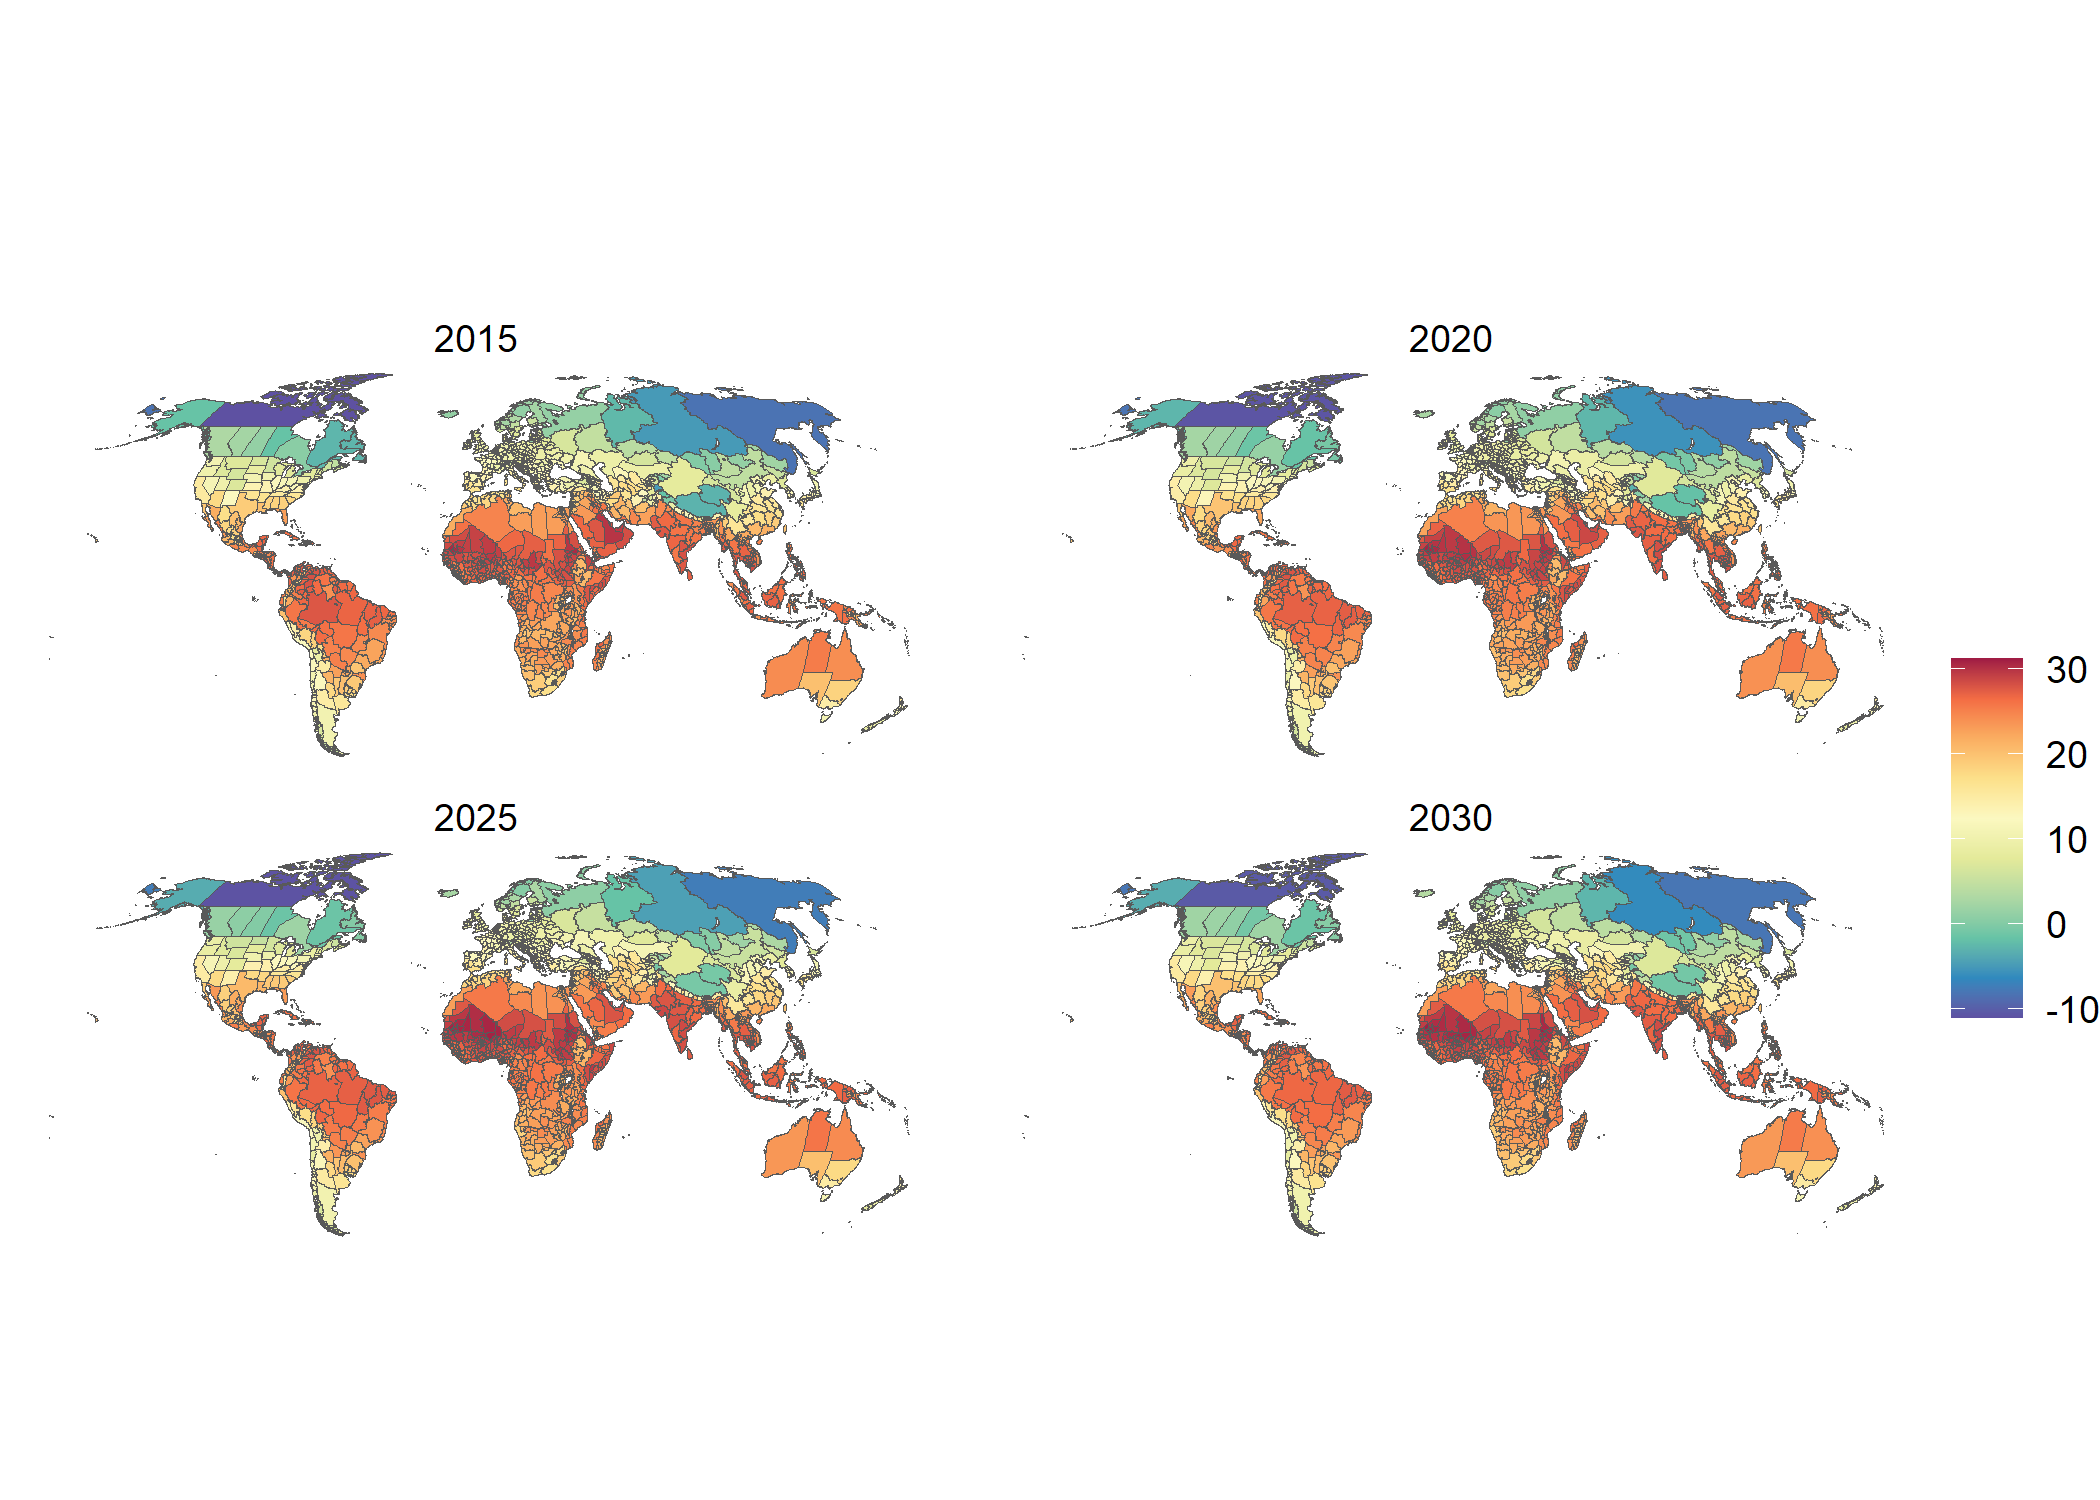
\includegraphics[width=\linewidth]{img/covars/tave.png}
  \caption{Mean temperature (Celsius)}
\end{figure}

\subsection{Topographic Ruggedness}
As a measure of accessibility, we include the mean topographic ruggedness of each admin area.  We first used a gridded dataset of elevation from the USGS \cite{USGS1996} and calculated the index at each grid cell using the methodology from Riley et al. \citep{Riley1999}.  We then summarized the values of all the grid cells within each administrative area.  Because this variable does not change over time, it is constant across all years in the model.

\begin{figure}[H]
  \centering
  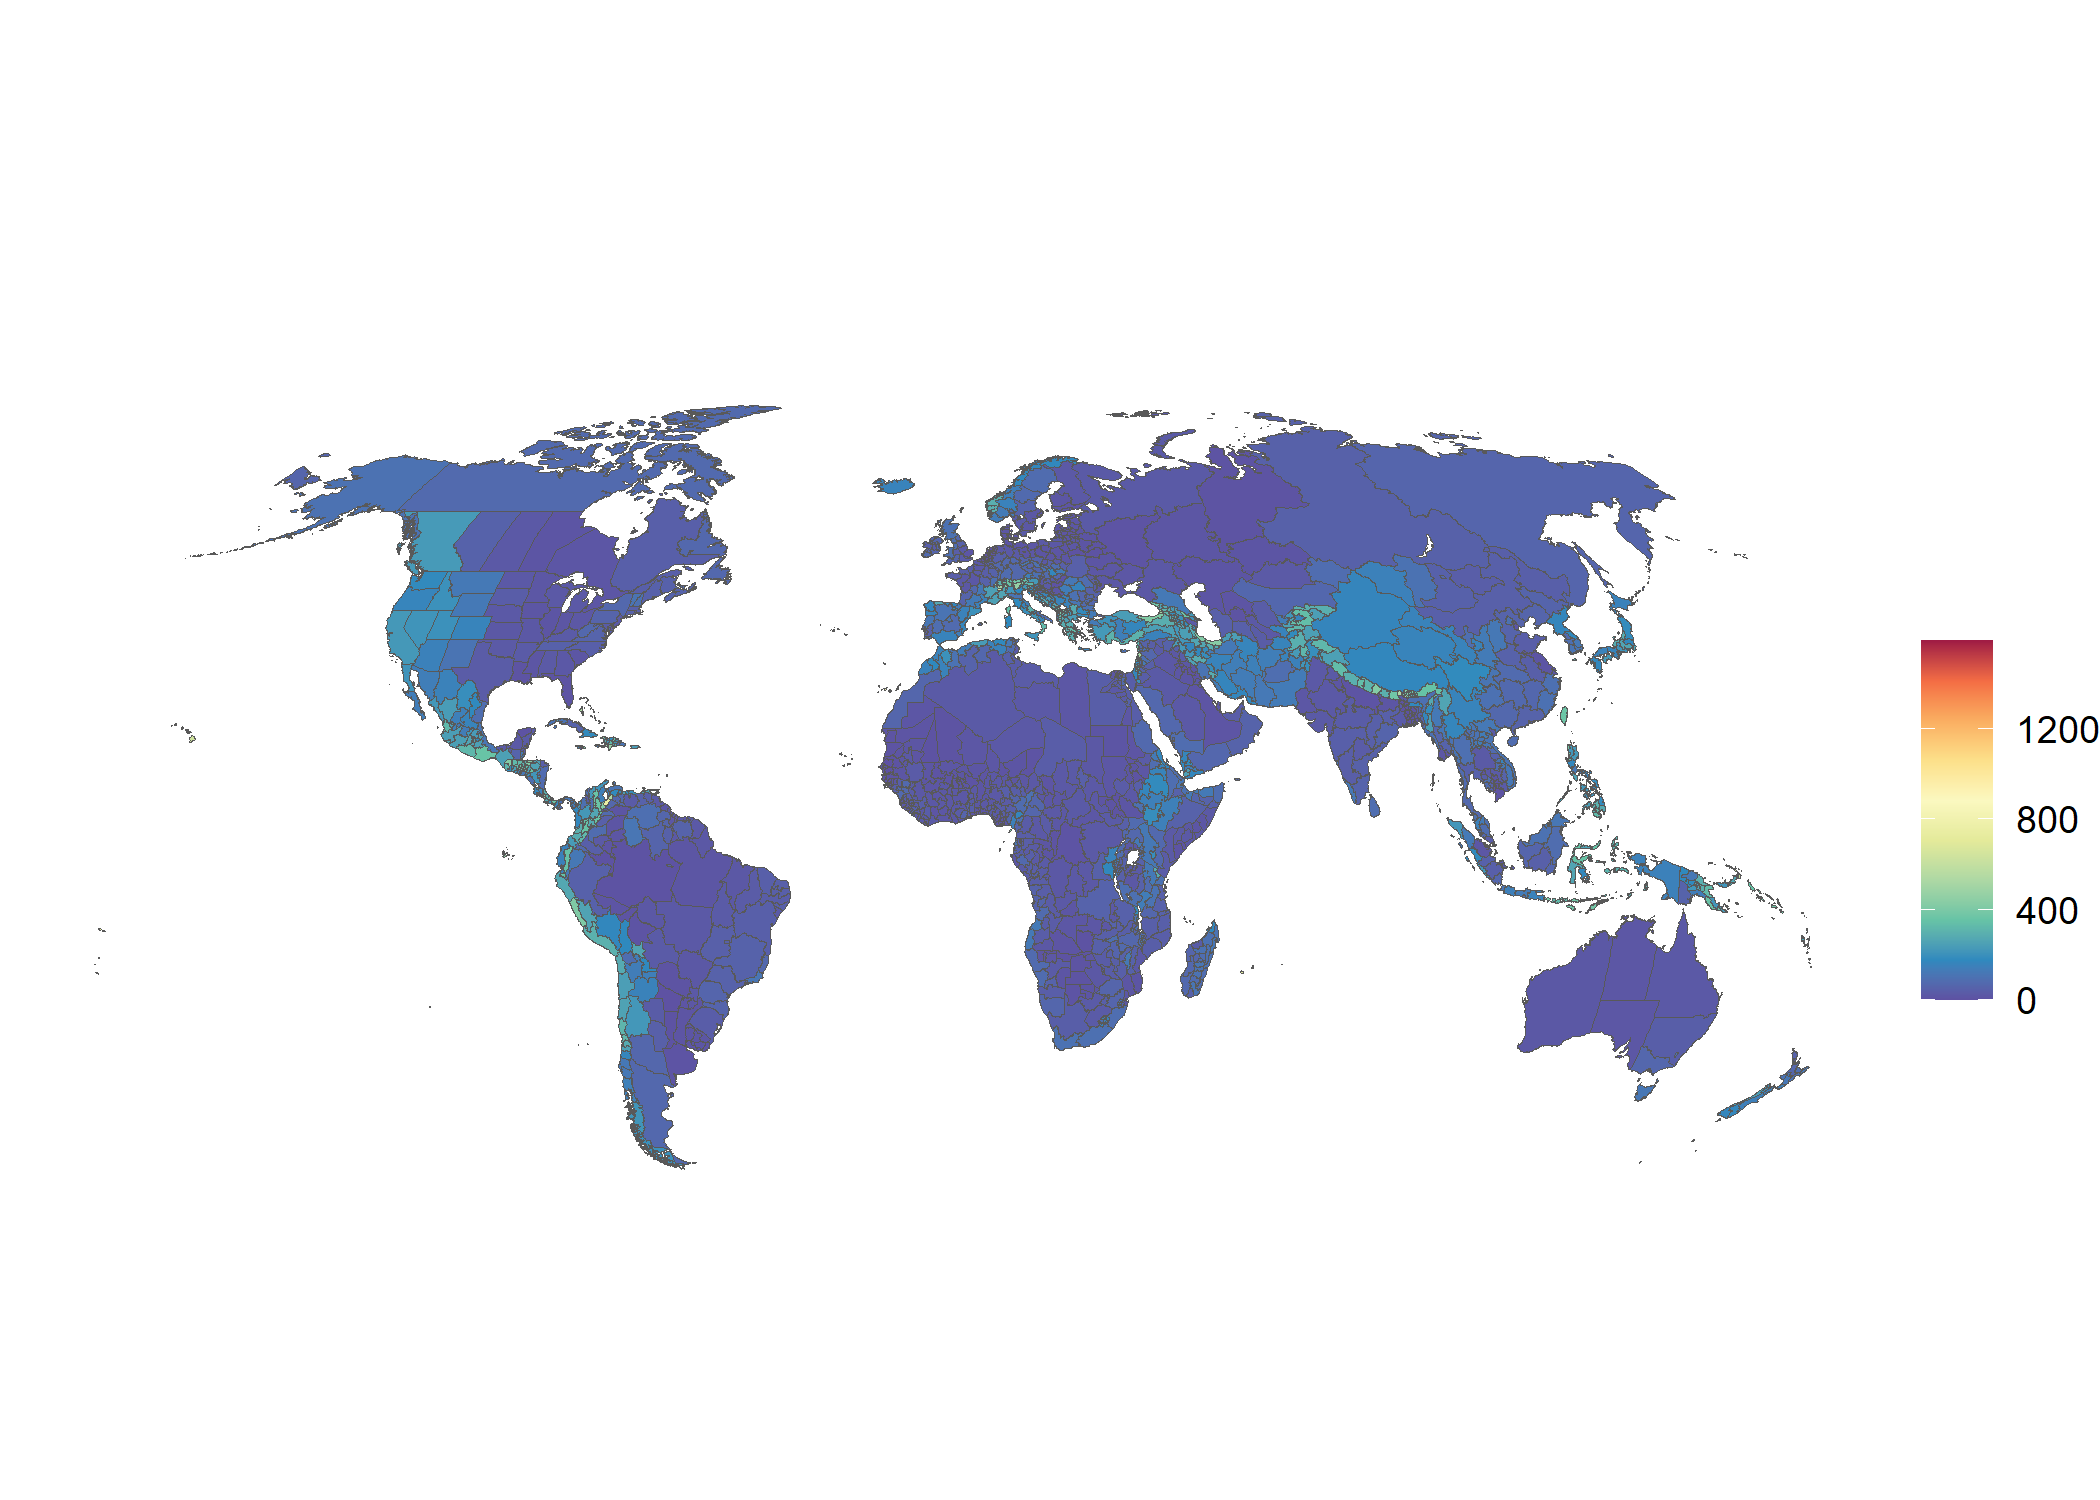
\includegraphics[width=\linewidth]{img/covars/ruggedness.png}
  \caption{Topographic ruggedness}
\end{figure}

\subsection{Malaria (\textit{P. falciparum}) Mortality Rate}
We used data from \textit{The Lancet} to estimate the mortality (deaths per 100,000 population per year) due to Malaria \citep{Weiss2019}, taking the average pixel values within each subnational administrative area.  We then estimated future malaria mortality based on AROC method.

\begin{figure}[H]
  \centering
  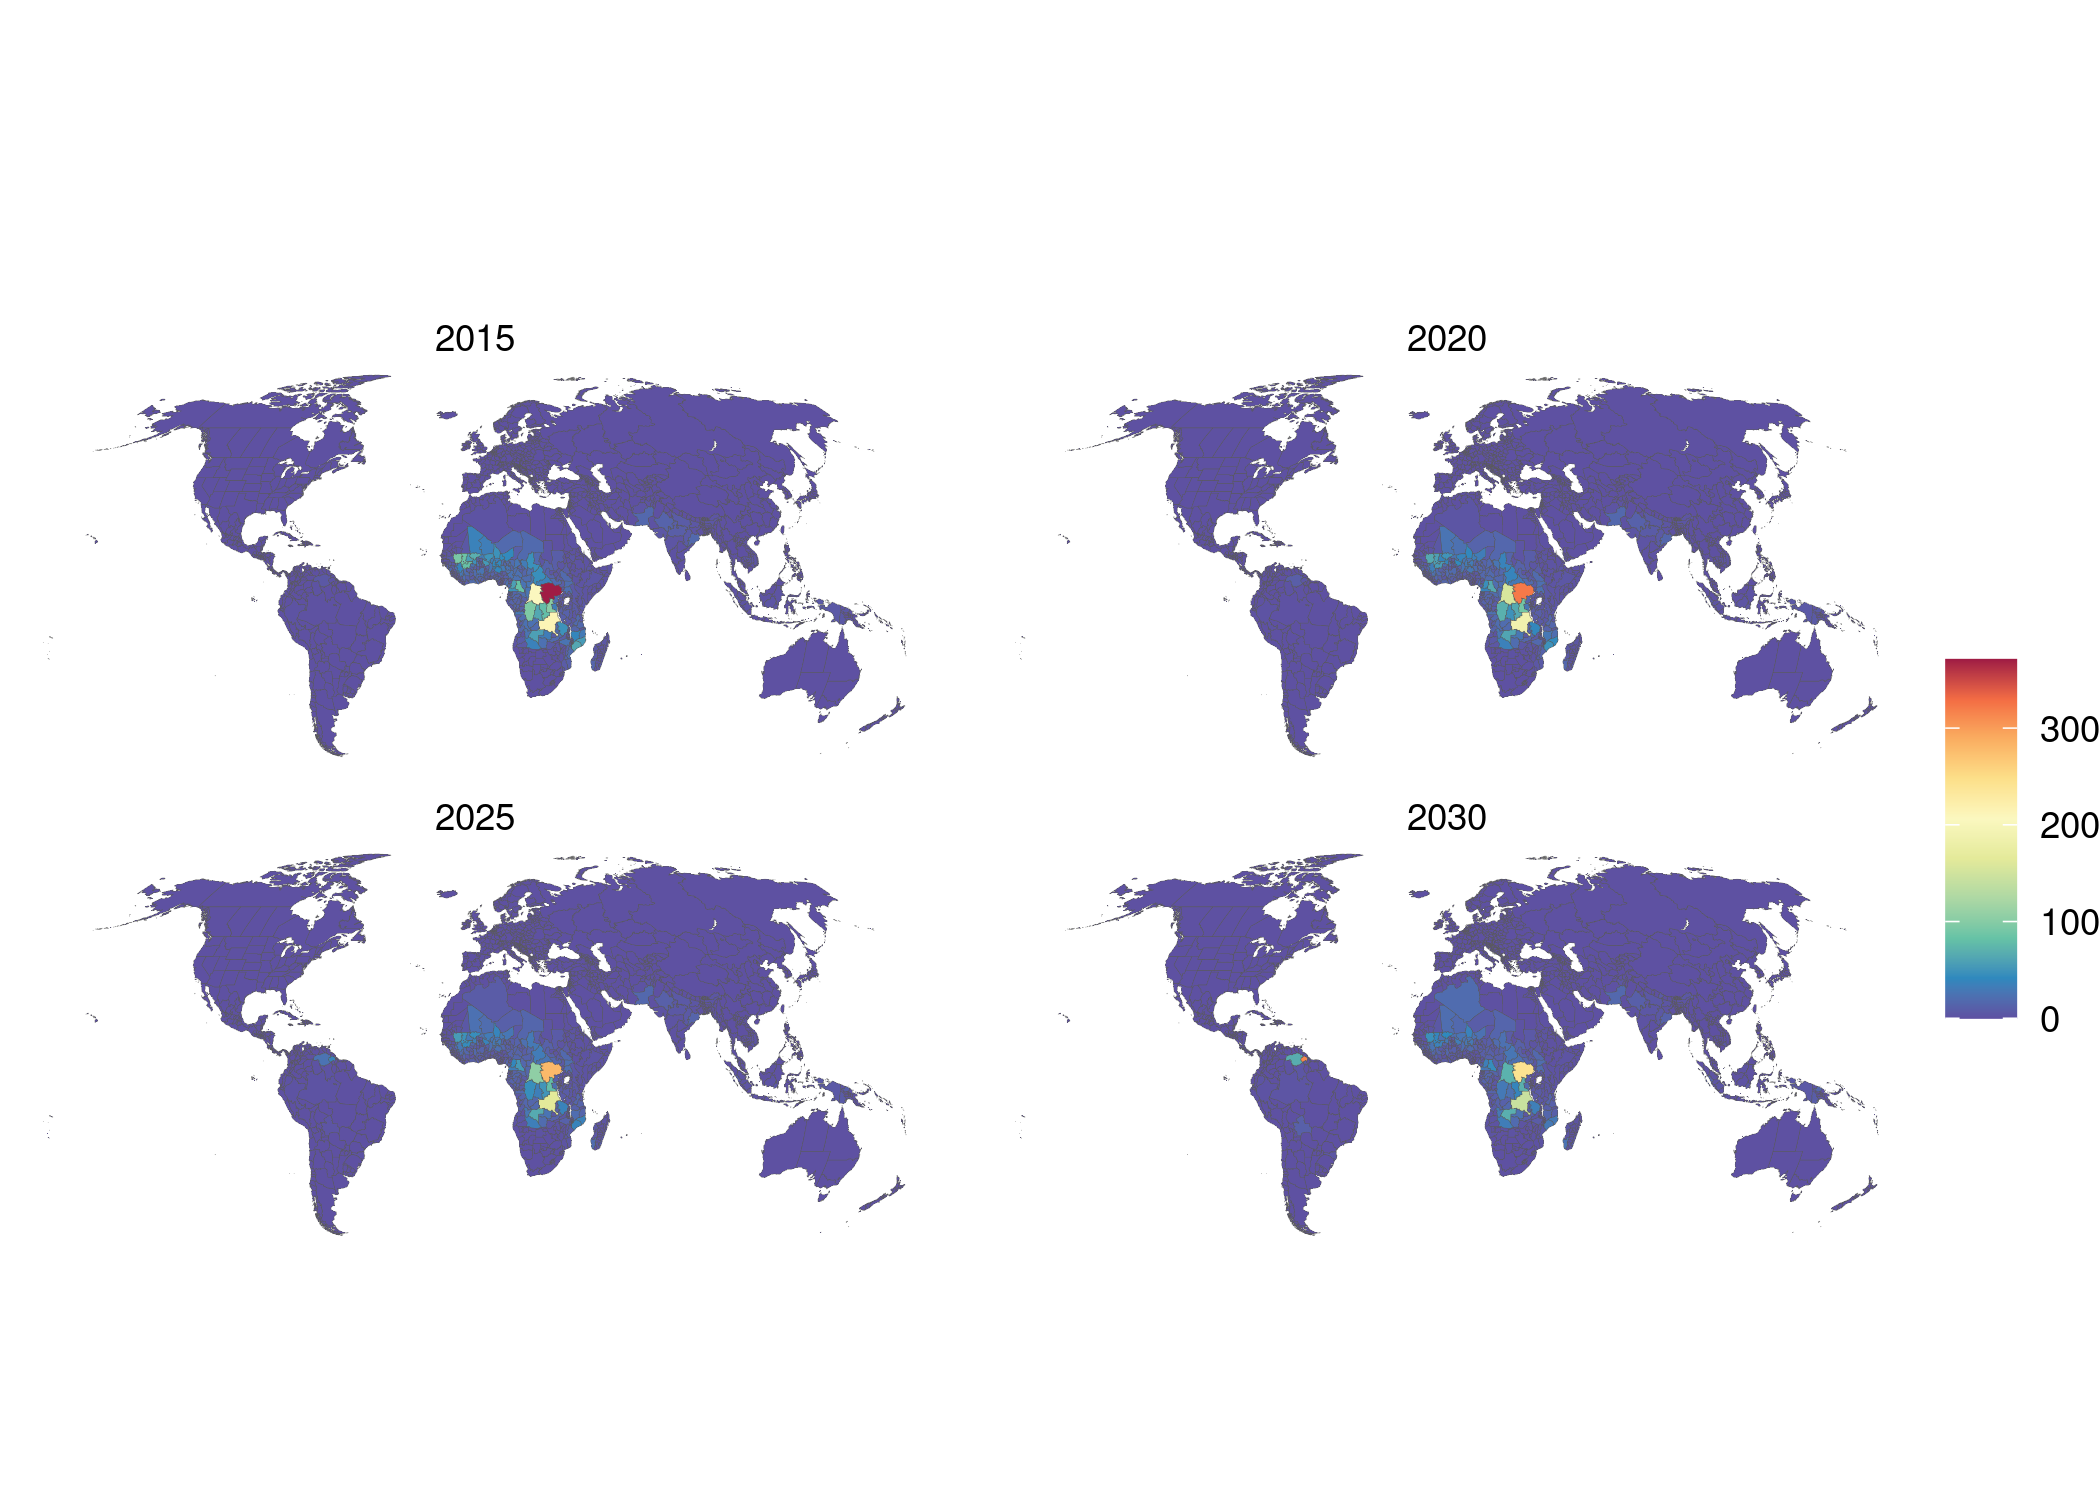
\includegraphics[width=\linewidth]{img/covars/mal_falciparum.png}
  \caption{Rate of mortality due to \textit{P. falciparum} Malaria}
\end{figure}

\section{Description, Implementation and Validation of the RF regression model}

%WE NEED HERE A SHORT PARAGRAPH ON HOW RF MODELS WORK, THIS WILL HELP: https://www.kdnuggets.com/2017/10/random-forests-explained.html
%INCLUDE BAGGING AND RANDOM FEATURE SELECTION, NECESSARY TO EXPLAIN OOB ERROR

The RF regression is a machine learning method based on the creation of a large number of decision trees. By taking an ensemble of decision tree models, random forests introduce more variance and balance out the bias that is common to single decision trees \citep{friedman2001elements}.  For each of the decision trees in a random forest model, observations are selected at random with replacement, a method known as bootstrap aggregating, or bagging, and features are area also selected at random.

For implementation we use the R-package \texttt{randomForestSRC} by Ishwaran and Kogalur \citep{ishwaran2019randomforestsrc}. Specifically, we apply the functions \texttt{tune.rfsrc()} to find the optimal combination of hyperparamters and the function \texttt{rfsrc()} to perform the RF regression models. After predicting rates of moderate-to-severe and severe food insecurity we plot the modeled vs. observed rates and calculated the MSE and ${R}^2$ (See Fig. \ref{fig:rf_in-sample} and Fig. \ref{fig:rf_out-sample}) for both models. Additionally, we use the function \texttt{vimp()} to gain insights into the development of the error rates with increasing numbers of trees (See Fig. \ref{fig:rf_error}) and the importance of individual variables (See Fig. \ref{fig:rf_vimp}).

%STEP-BY-STEP: LOGIT TRANSFORM, TUNE, MODEL, PREDICT, VALIDATE

To ensure that predicted rates are bounded by 0 and 1 we conduct a logit transformation of the dependent variable and inverse logit transformation of the predictions. 
%MAYBE STATE THIS SOMEWHERE ELSE, NOT SURE WHERE

\begin{figure}[H]
  \centering
  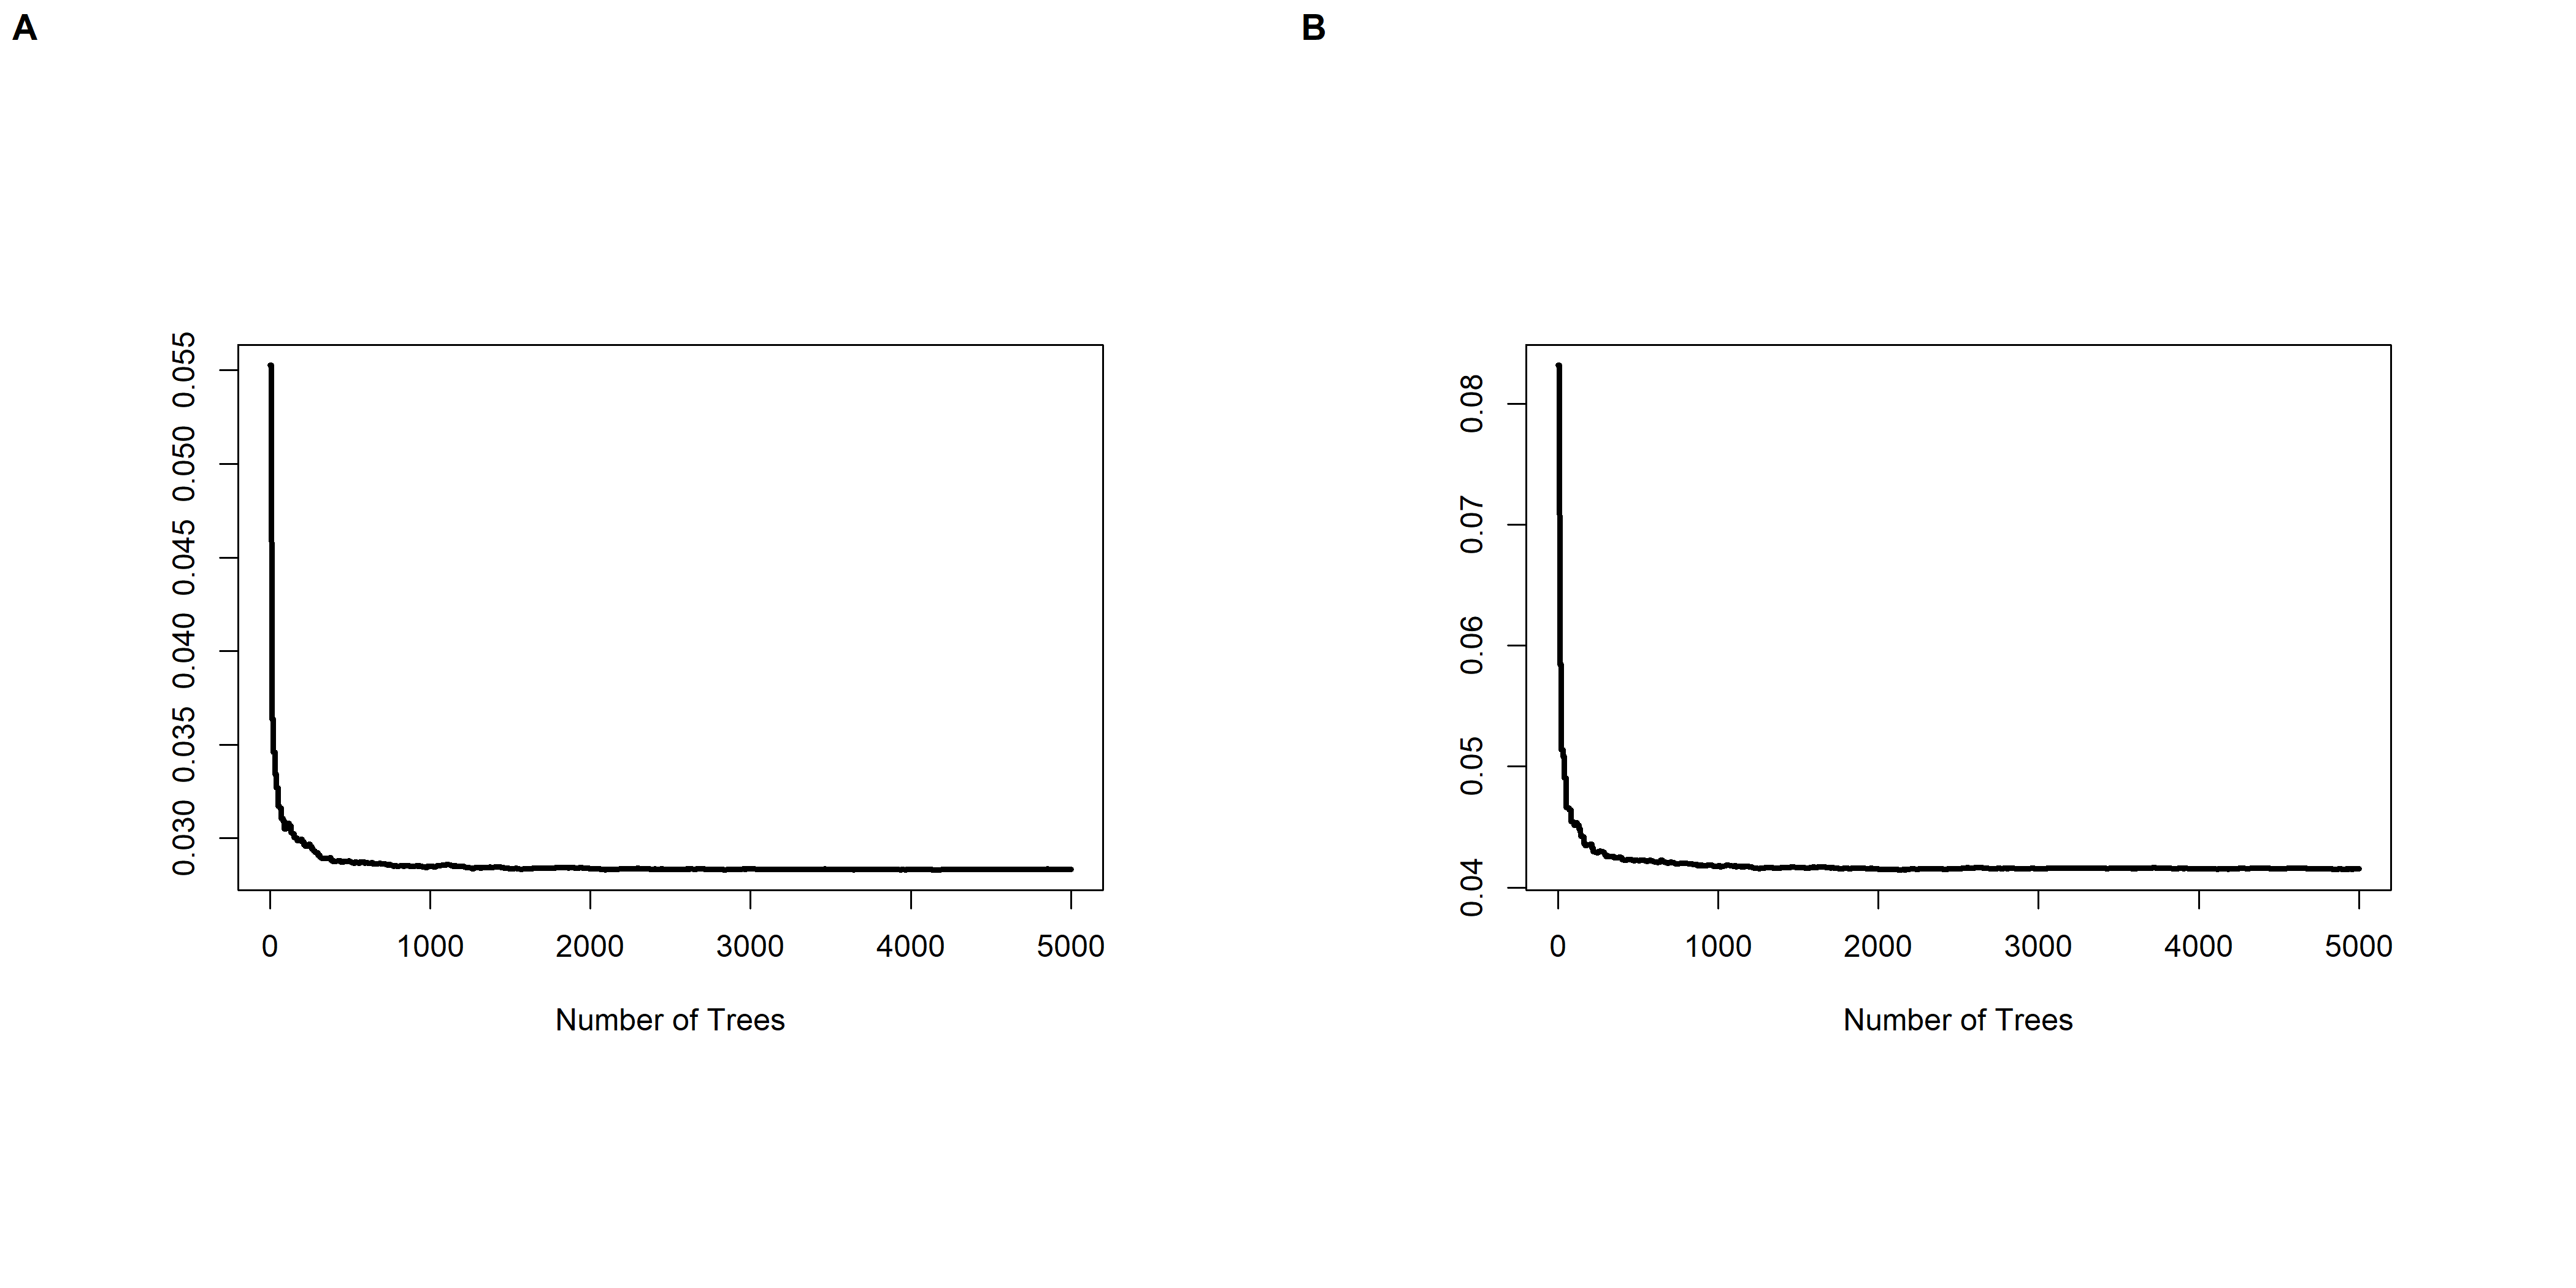
\includegraphics[width=\linewidth]{img/model/error_rf.png}
  \caption{Error Rate of the RF regression model. Panel (A) shows the Moderate-to-Severe model and Panel (B) shows the Severe model.}
  \label{fig:rf_error}
\end{figure}

%HERE A FEW SENTENCES ON THE NUMBER OF TREES WITH LINK TO NEXT PARAGRAPH

In addition to the parameter that describes the number of trees to be created, two other important hyperparameters must be tuned. In the function \texttt{tune.rfsrc()} these parameters are called \texttt{mtry} and \texttt{nodesize}. \texttt{mtry} describes the number of variables randomly selected as candidates for splitting a node and \texttt{nodesize} describes the average number of observations in a leaf node. The optimal pair of hyperparamters is found by trying different combinations and choosing the one with the smallest out-of-bag (OOB) error.

%EXPLAIN THE OOB ERROR HERE?

The function \texttt{tune.rfsrc()} does exactly that and returns optimal values for \texttt{mtry} and \texttt{nodesize}. We applied this function on the both, the moderate-to-severe and the severe model. For the moderate-to-severe model the optimal combination is \texttt{mtry} = 12 and \texttt{nodesize} = 1 and for the severe model we found \texttt{mtry} = 10 and \texttt{nodesize} = 2 to be optimal.

%STATE FUNCTION ARGUMENTS HERE?

\begin{figure}[H]
  \centering
  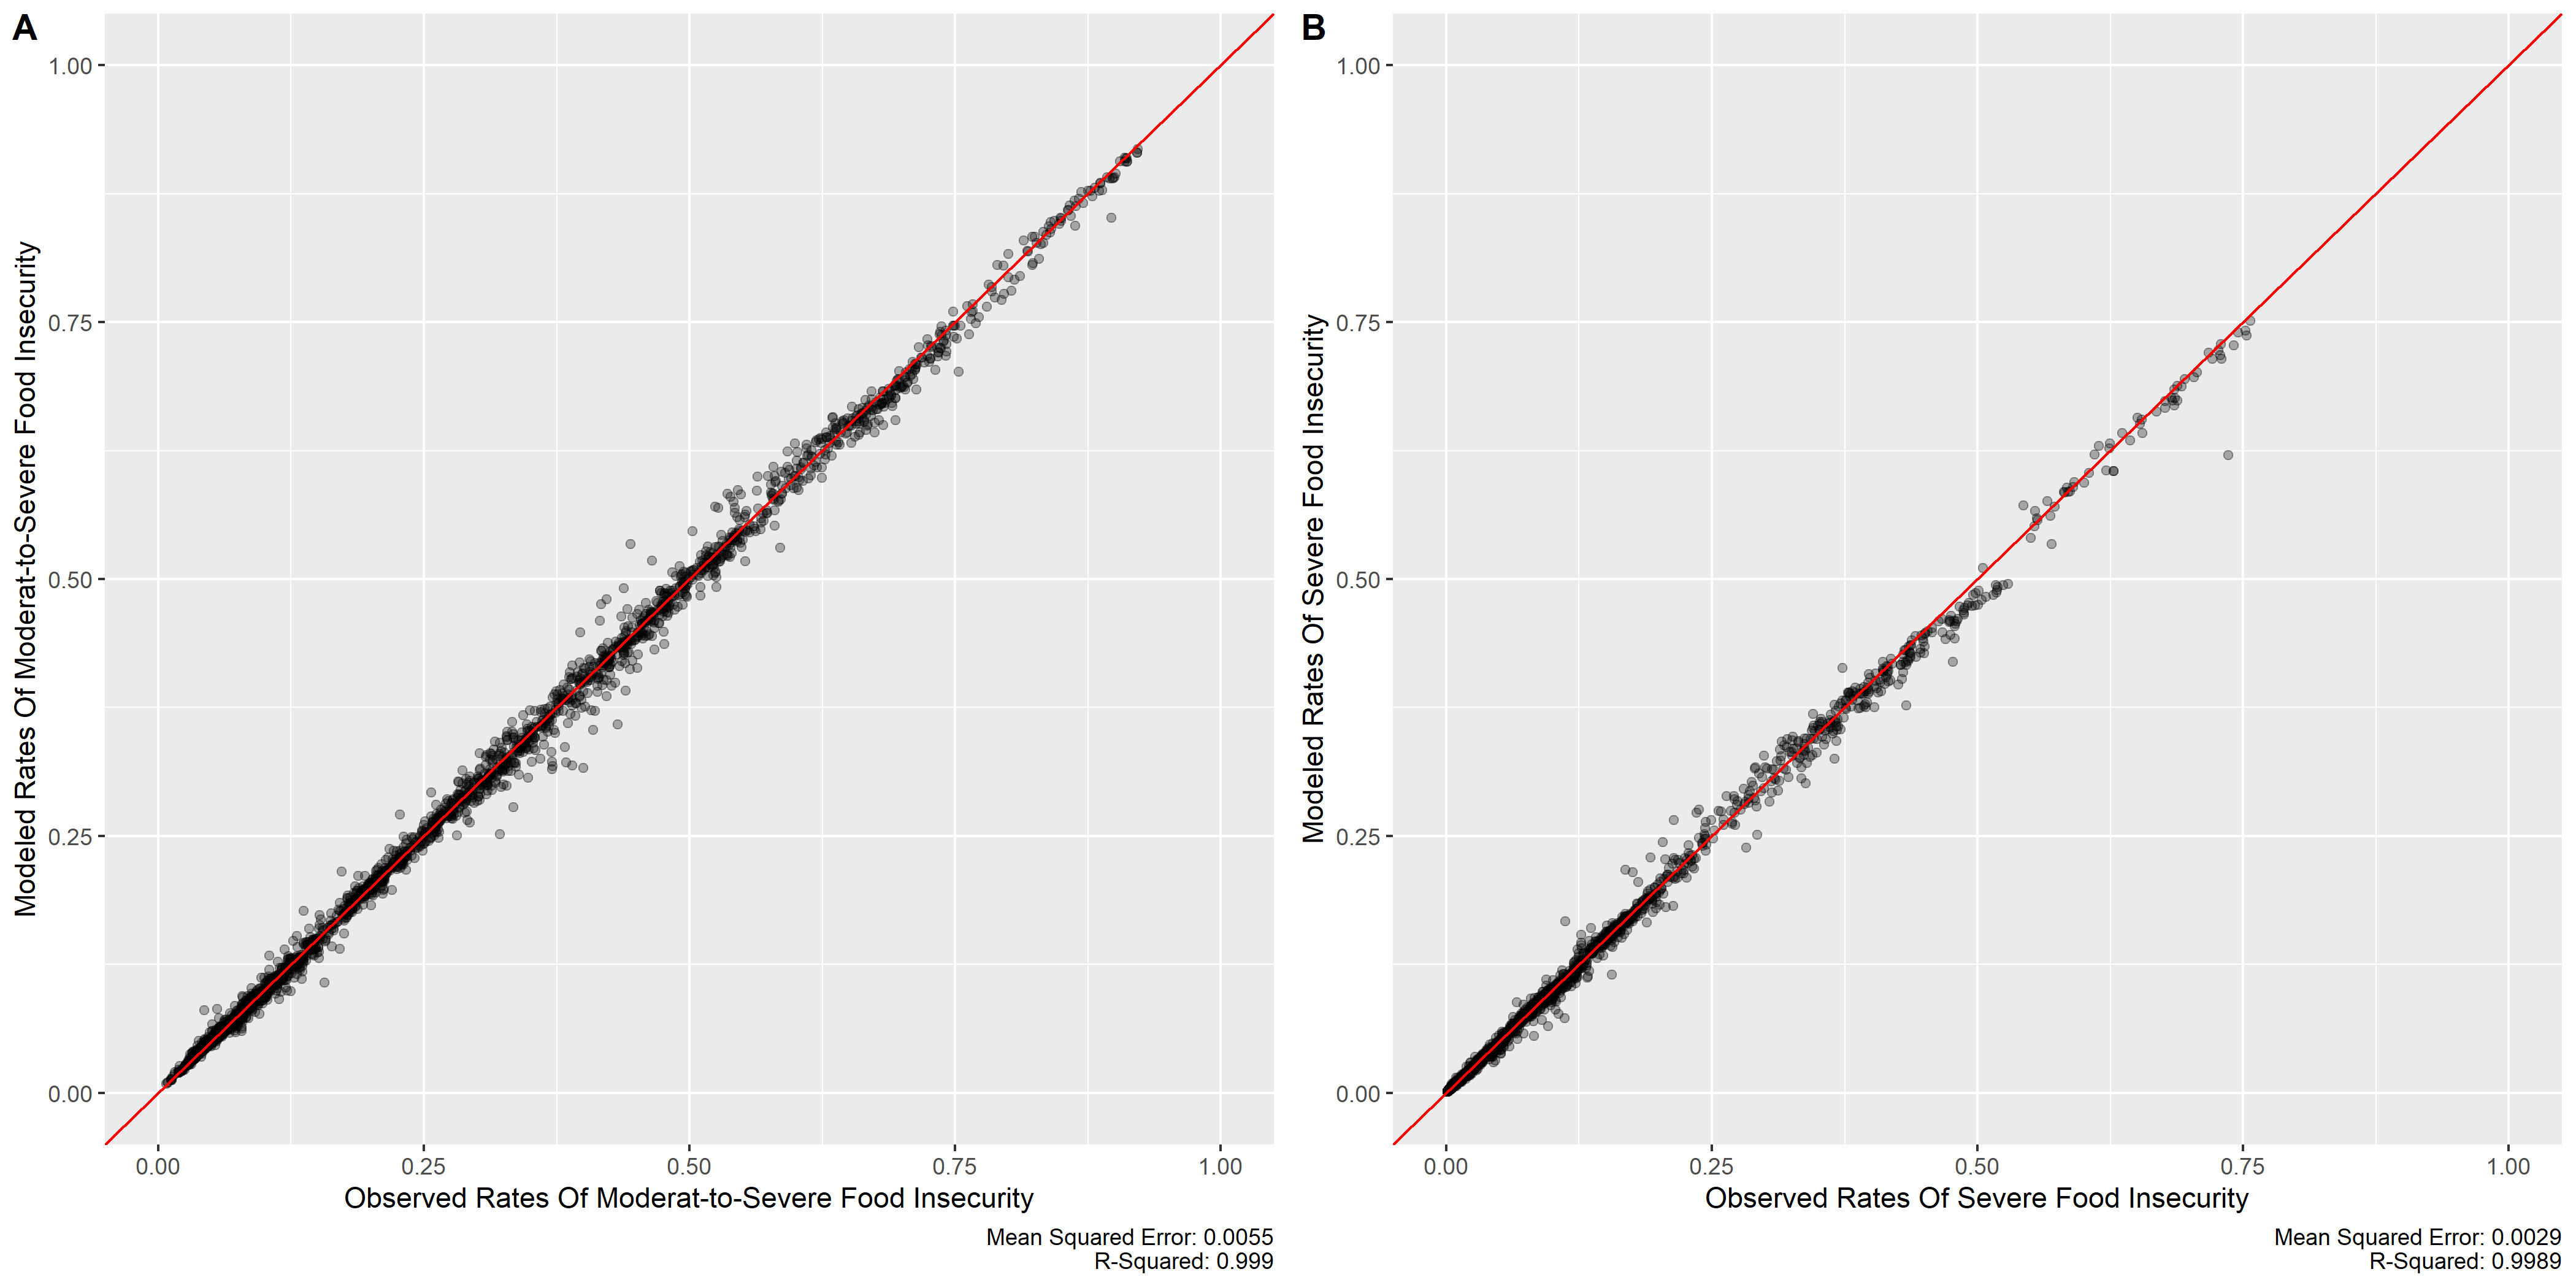
\includegraphics[width=\linewidth]{img/model/in-sample_rf.png}
  \caption{In-Sample Fit of the RF regression model. Panel (A) shows the Moderate-to-Severe model and Panel (B) shows the Severe model.}
  \label{fig:rf_in-sample}
\end{figure}

\begin{figure}[H]
  \centering
  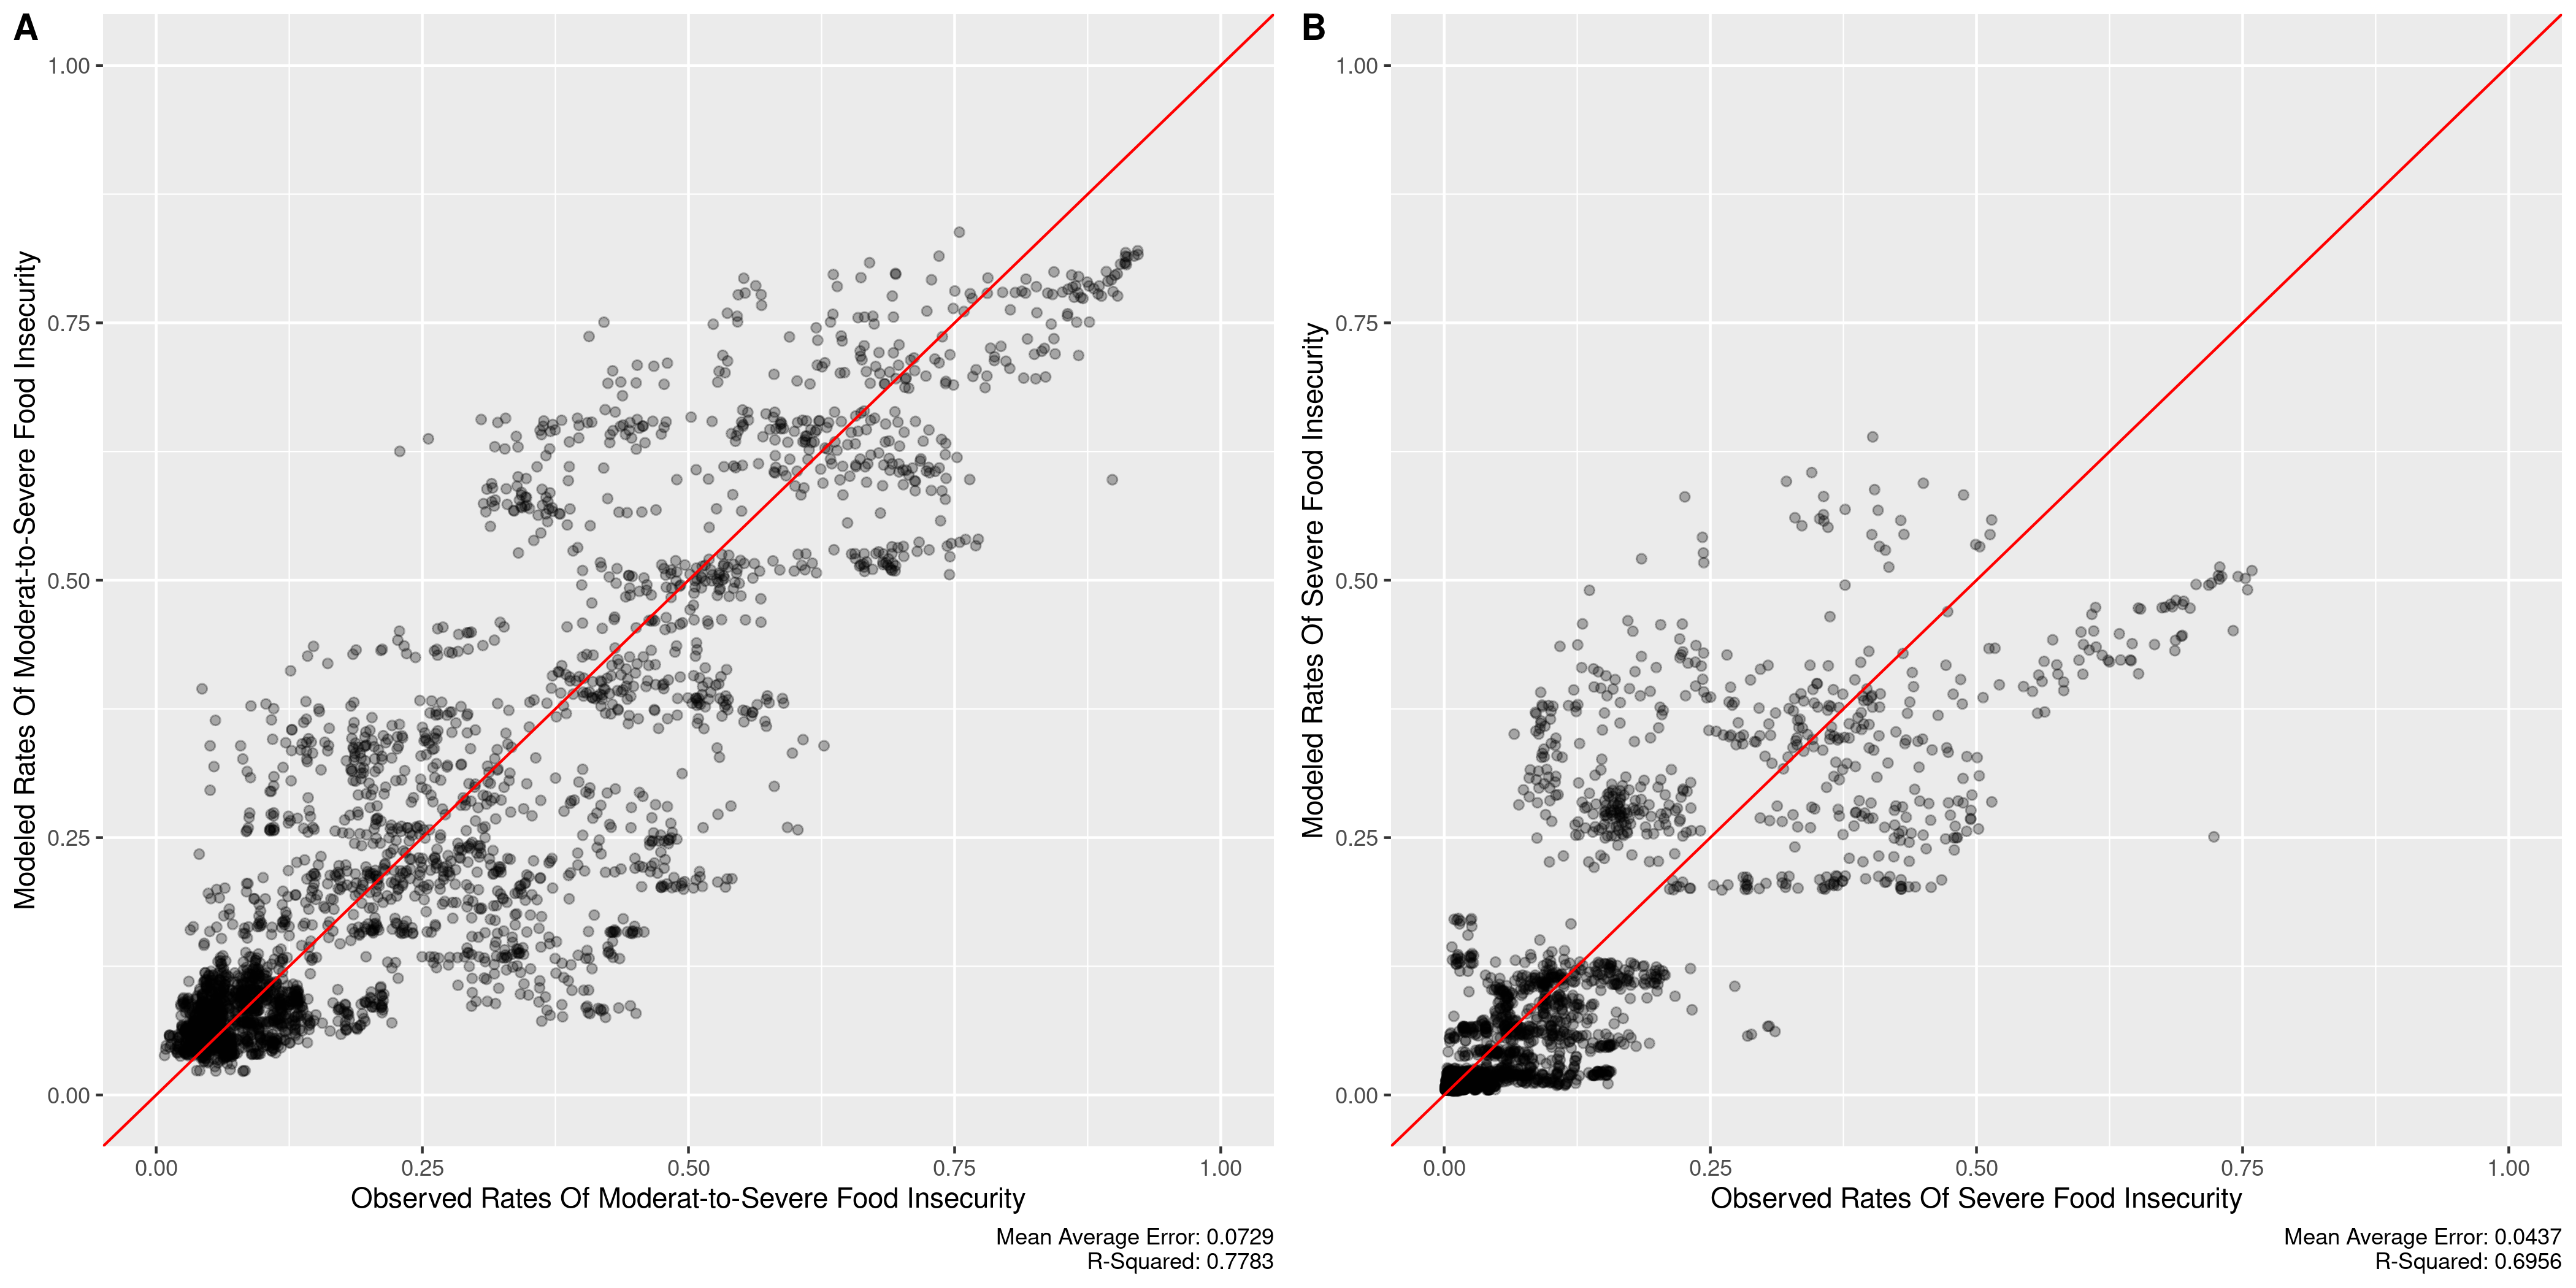
\includegraphics[width=\linewidth]{img/model/out-sample_rf.png}
  \caption{Out-Of-Sample Fit of the RF regression model with 75\% training set and 25\% test set. Panel (A) shows the Moderate-to-Severe model and Panel (B) shows the Severe model.}
  \label{fig:rf_out-sample}
\end{figure}

%HERE EVERYTHING ON THE MODEL, NOT SURE HOW DETAILED
%For modeling the rates of moderate-to-severe and severe food insecurity we use the function \texttt{rfsrc()}. We specify 

\begin{figure}[H]
  \centering
  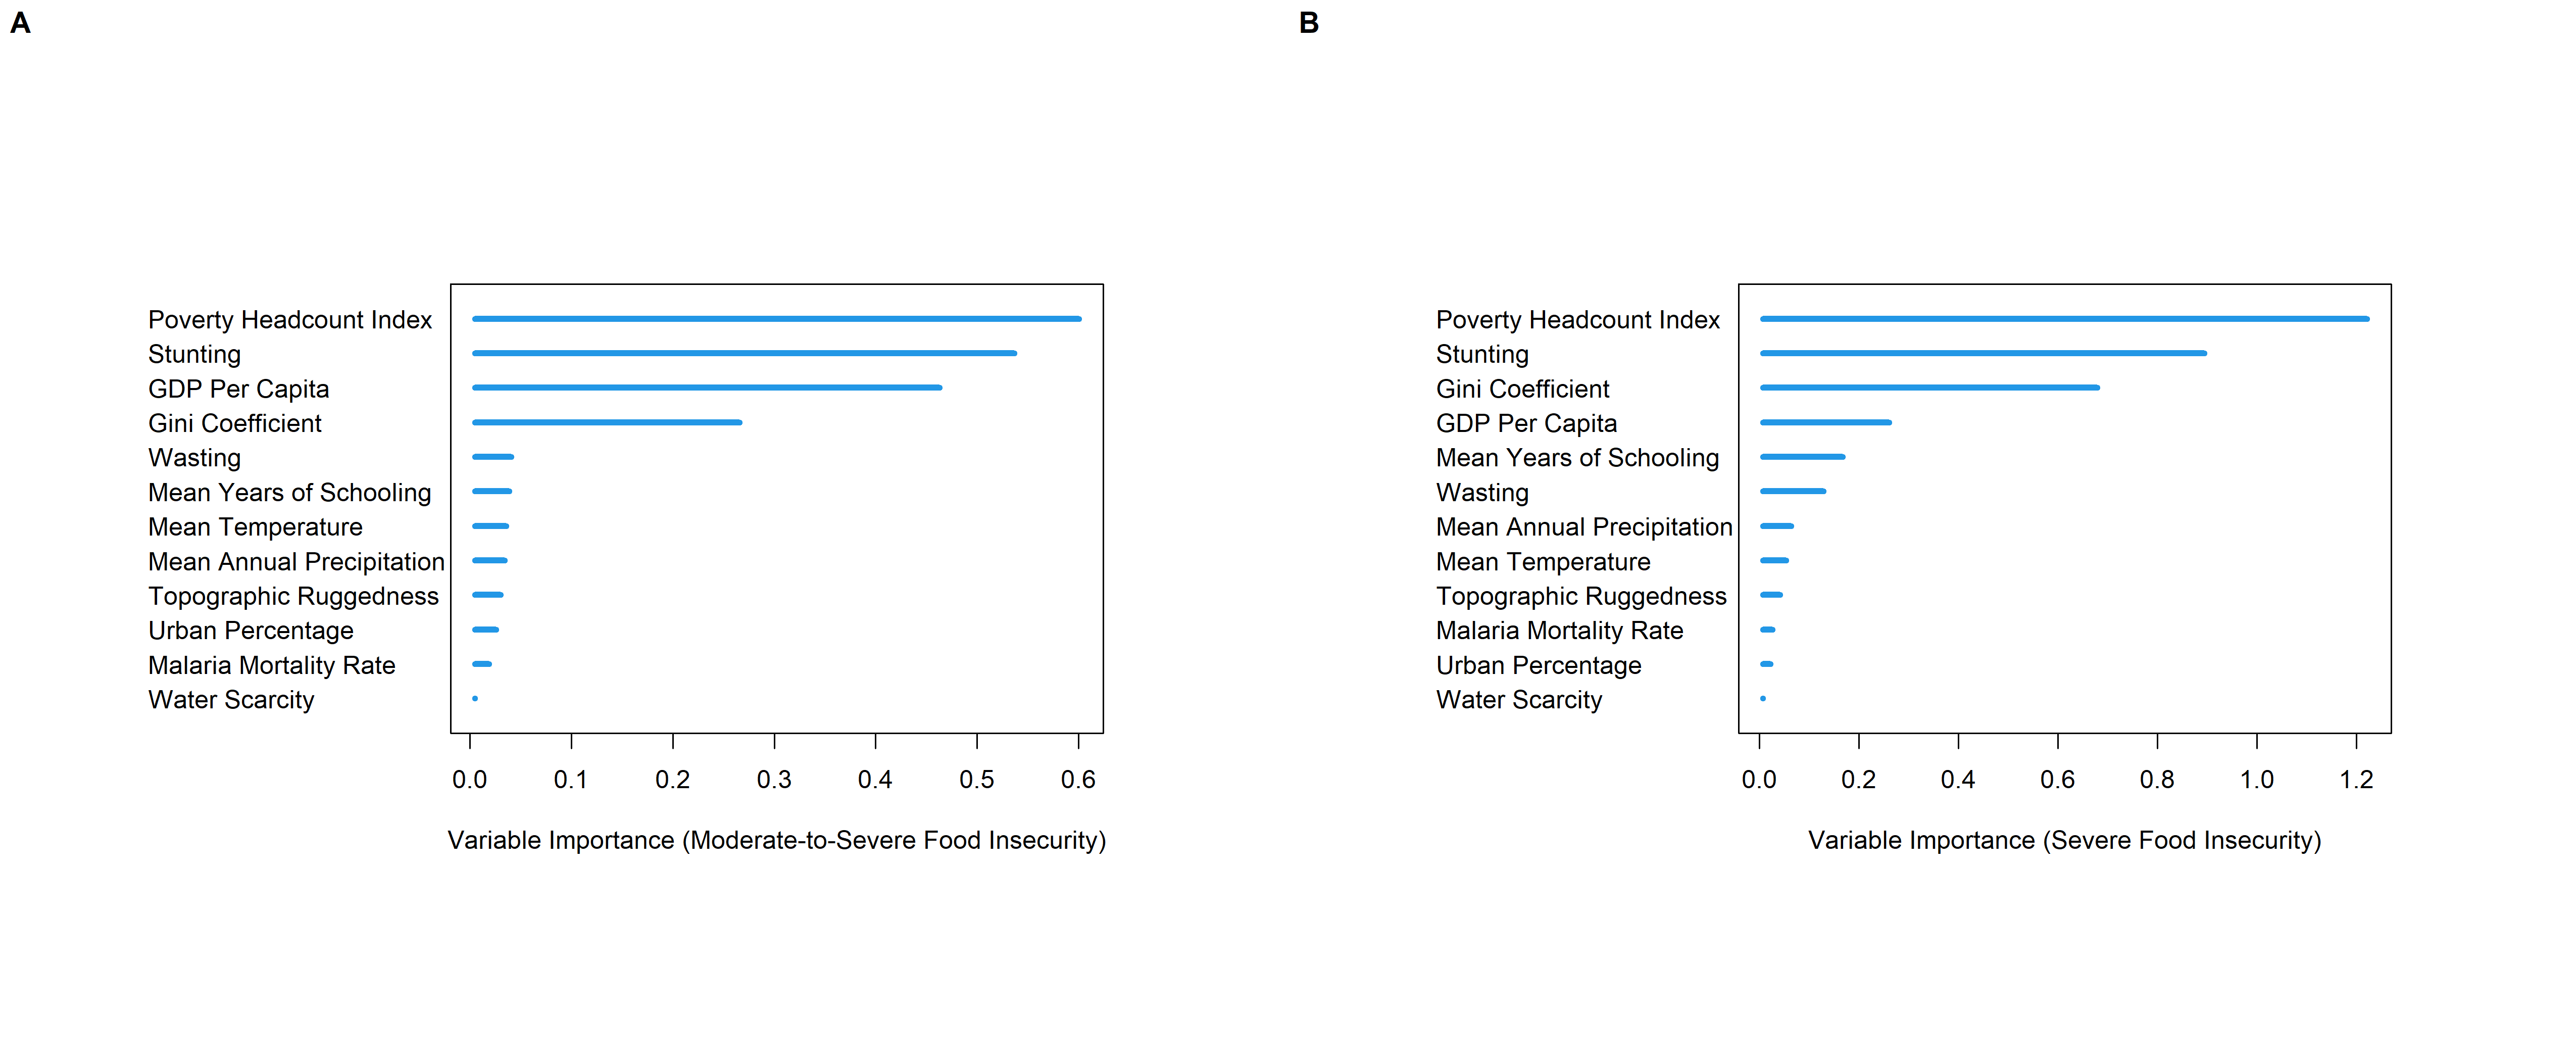
\includegraphics[width=\linewidth]{img/model/vimp_rf.png}
  \caption{Variable Importance of the RF regression model. Panel (A) shows the Moderate-to-Severe model and Panel (B) shows the Severe model.}
  \label{fig:rf_vimp}
\end{figure}

%https://kogalur.github.io/randomForestSRC/theory.html#section4.2
Lastly we asses the importance of individual variables. This is based on the Breiman-Culter permutation variable importance information \citep{breiman2001random}.  This involved comparing the prediction error on the OOB data to the prediction error of OOB cases where the x-variable $x$ is randomly permutated.  The importance of an individual variable is thus the mean difference between the perturbed and unperturbed error rate, across all trees. 
%MORE INFORMATION HERE




\end{document}
